%------------------------------------------------------------------------------
\chapter{1-D Space discretization}\label{sec:1d_space_discretization}
We are looking for a second order central space discretization together with the finite volume approach.
So the higher order terms in the Taylor series expansion are negligible.
For this numerical discretization method no dissipation is added, only there is some dispersion for the shorter waves, i.e.\ dependent on the third derivative in the Taylor expansion.
To fulfill this requirement the data should be smooth according to the truncation error of the numerical discretization.
If not, the data should be made smooth with a procedure in which you can see on which location the smoothing is severe.
The process of smoothing is called regularization.
If the truncation error (high values of second derivatives) is severe on locations that the user do not expect and do not accept then the user can adjust the discretization in that part of the domain.
%
There are two options to adjust the data:
\begin{enumerate}
    \item increase the smoothing coefficient or
    \item choose a smaller grid size.
\end{enumerate}

%------------------------------------------------------------------------------
\section{Finite volume approach}
We will discuss the finite volume approach for the one dimensional case of the function $u(x,t)$,
for the grid shown in  \autoref{fig:water_body_fve_bc_at_node}
\begin{figure}[H]
    \centering
    \begin{center}
    \resizebox{0.8\textwidth}{!}{
        \input{figures/water_body_fve_bc_at_node.pdf_tex}
    }
\end{center}
    \caption{Water body (blue area), finite volumes (green boxes), computational points (open dots), virtual computational points (black dots), boundary points (open squares) are at $i=1$ (west boundary) and $i=I$ (east boundary).}\label{fig:water_body_fve_bc_at_node}
\end{figure}
The control volume is defined on the interval $x_{i-\half}$ to $x_{i+\half}$, see \autoref{fig:water_body_fve_bc_at_node}.
The grid in \autoref{fig:water_body_fve_bc_at_node} is equidistant but that is not necessarily, the method which is described in this document also holds for a non-equidistant grid.

%------------------------------------------------------------------------------
\subsection{Quadrature rule, source term}\label{sec:source_quadrature_rule}
The finite volume approach for the function $u(x,t)$ reads:
\begin{align}
    \int_\Omega u \, d\omega = \int_{x_{i-\half}}^{x_{i+\half}} u \, dx
\end{align}
Using piecewise linear functions between the non-equidistant nodes the quadrature rule reads:
\begin{align}
    \int_{x_{i-\half}}^{x_{i+\half}} u \, dx & = \int_{x_{i-\half}}^{x_i} u \, dx + \int_{x_i}^{x_{i+\half}} u \, dx \approx
    \\
    & \approx \frac{\Dx_{i-\half}}{2} \frac{u_{i-1} + 3 u_{i}}{4} + \frac{\Dx_{i+\half}}{2} \frac{3 u_{i} + u_{i+1}}{4} \label{eq:integral_control_volume}
\end{align}
where the control volume is split into two adjacent sub-control volumes  $[x_{i-\half}, x_i]$ and $[x_i, x_{i+\half}]$.
A graphical interpretation is given in \autoref{fig:1d_integration_1points_gauss}.
\begin{figure}[H]
        \begin{center}
            \resizebox{0.9\textwidth}{!}{
                \import{figures}{1d-integration_1_points_gauss.pdf_tex}
            }
        \end{center}
    \caption{Integration of a quadratic function at $x_i$ over the control volume from $x_{i-\half}$ to $x_{i+\half}$. 1-point Gauss is exact for linear functions but not for quadratic functions.}\label{fig:1d_integration_1points_gauss}
\end{figure}
Higher order quadrature rules may be chosen, but they are not discussed in this report.
%\begin{figure}[H]
%    \begin{subfigure}{0.475\textwidth}
%       \begin{center}
%        \def\svgwidth{1.2\textwidth} % scaling text
%        \resizebox{0.9\textwidth}{!}{
%            \import{figures}{1d-integration_1_points_gauss.pdf_tex}
%        }
%    \end{center}
%    \caption{Quadratic function approximated by 1-point Gauss.} \label{fig:1d_integration_1points_gauss}
%    \end{subfigure}
%\hfill
%    \begin{subfigure}{0.475\textwidth}
%    \begin{center}
%        \def\svgwidth{1.2\textwidth} % scaling text
%        \resizebox{0.9\textwidth}{!}{
%            \import{figures}{1d-integration_2_points_gauss.pdf_tex}
%        }
%    \end{center}
%    \caption{Quadratic function approximated by 2-point Gauss.} \label{fig:1d_integration_2points_gauss}
%    \end{subfigure}
%    \caption{Integration of a quadratic function over the control volume  $[x_{i-\half}, x_{i+\half}]$. 1-point Gauss is exact for linear functions but not for quadratic functions, 2-points Gauss is exact for linear, quadratic and cubic functions.} \label{fig:1d_integration}
%\end{figure}

%------------------------------------------------------------------------------
\subsection{Quadrature rule, flux term}\label{sec:flux_quadrature_rule}
\notyet
%------------------------------------------------------------------------------
\subsection{Boundary conditions}\label{sec:boundary_conditions}
At the west and east boundary boundary conditions need to be supplied.
If it is a prescribed boundary condition (ingoing signal) it is called an \textbf{essential}-boundary condition, if the boundary condition is determined by the outgoing signal it is called a \textbf{natural}-boundary condition \citep{Logan1987,VanKanEtAL2008}.
In case of a wave equation we have a right and left going signal.
When no reflection at an open boundary is required then at the west boundary a signal need to prescribed  without disturbing the left going signal.
And at the east boundary the other way around.

Further more we have the prescribed boundary signal at the boundary node of the grid.
This assumption is made because the users are acquainted with the fact that open boundaries are given at nodes.
But for the outgoing signal this is not necessarily, for the outgoing signal we stick to the finite volume approach.

When we consider a one dimensional right going signal (see \autoref{sec:1d_adv_diff_equation}) the boundary at the west side is located at $x_1$ and the outflow condition is located at $x_{I+\half}$.
The prescribed function reads:
\begin{align}
    c(0,t) = f(t)
\end{align}
Because we use a 3-point stencil for the interior, we aim for a 3-point stencil for the essential boundary condition.
One possible quadratic interpolation is a parabolic fit through the grid points, giving an under specification of the solution at the boundary regardless of its position.
\begin{align}
    c_{GP}(\xi) & = c_0 \,  (1 - \xi) + c_1 \,  \xi + \half(c_0 - 2\, c_1 + c_2) \,  (\xi - 1) \,  \xi
    =
    \nonumber \\
    & =  \left(1 - \xi\right) \,  \left(1 - \half \xi\right) c_0  + \xi \,  \left(2 - \xi\right) c_1 + \half \xi  \left(\xi - 1\right) \,  c_2
    \label{eq:20231214-1}
\end{align}
where $\xi\in [0,1]$ is the weight function between $c_0$ and $c_1$.

Another possible quadratic fit is the one through Cell-Centered values:
\begin{align}
    c_{CC}(\xi) & = c_0 \, \left(1 - \xi\right) + c_1\,  \xi + \half (c_0 - 2c_1 + c_2) \,   \left(\xi - \half\right)^2
    \\
    & = \left( 1 - \xi + \half \left(\xi - \half\right)^2 \right) c_0 +
    \left( \xi - \left(\xi - \half\right)^2  \right) c_1  +
    \left(   \half \left(\xi - \half\right)^2\right) c_2       \label{eq:20231214-5}
\end{align}
The parabolic fit that gives neither underspecification nor overspecification of
imposed values at boundaries is a combination of Equation (45) and (49).
It is easy to show that that combination consists of $1/3$ times \autoref{eq:20231214-1} plus $2/3$ times \autoref{eq:20231214-5}:
\begin{align}
    c_{opt}(\xi) & = \left( \frac{13}{12} - \frac{3}{2}\xi - \half \xi^2 \right) c_0 +
    \left( -\frac{1}{6} + 2 \xi - \xi^2 \right) c_1  +
    \left( \frac{1}{12} - \half \xi +  \half \xi^2  \right) c_2
\end{align}
Which lead to the following interpolations for $\xi=\half$ and $\xi=1$:
\begin{align}
    c_{opt}\left(\half\right) & = \frac{11}{24} c_0 + \frac{14}{24} c_1 - \frac{1}{24} c_2 \label{eq:stencil_nat}
    \\
    c_{opt}\left(1\right)  & = \frac{1}{12} c_0 + \frac{10}{12} c_1 + \frac{1}{12}c_2 \label{eq:stencil_ess}
\end{align}
Where \autoref{eq:stencil_nat} will be used for the natural boundary condition and \autoref{eq:stencil_ess} will be used for the essential boundary condition.

Verification of its correctness by means of integration over the outermost finite volume:
\begin{align}
\int_{\xi_{\half}}^{\xi_{\frac{3}{2}}} c_{opt}(\xi)\, d\xi = \frac{1}{8} c_0 + \frac{3}{4} c_1 + \frac{1}{8} c_2
\end{align}
In the right-hand side we see the weights of the mass matrix of the piecewise linear FVE
method, i.e.\ averaged over the left outermost finite volume the quadratic function $c_{opt}$
equals the piecewise linear function used in the FVE scheme.
%------------------------------------------------------------------------------
%\newpage
\section{Regularization of artificial viscosity $\mathbf{\Psi}$}\label{sec:regularization_artificial_viscosity}
To get an error-minimizing method we need to regularize all data, as mentioned in \autoref{sec:error_minimizing}.
Regularization of the artificial viscosity $\Psi$ is performed as described in \citet[eq.\ 14]{Borsboom2001}.
\begin{align}
    \int_\Omega \Psi\, d\omega - \alpha_{\psi} \int_\Omega \Dxi^2 \pdiff[2]{\Psi}{\xi}\, d\omega = \int_\Omega \beta_{\psi} Err_{\beta_{\psi}}\, d\omega
\end{align}
When discretized it yields \citep[eq.\ 18]{Borsboom2001}:
\begin{align}
    \left(\frac{1}{8} - \alpha_{\psi} \right)\Psi_{i-1} +
    \left(\frac{3}{4} + 2\alpha_{\psi} \right)\Psi_{i} +
    \left(\frac{1}{8} - \alpha_{\psi} \right)\Psi_{i+1} = \frac{\beta_{\psi}}{\Dxi} \int^{\xi_{i+\half}}_{\xi_{i-\half}} Err_{\beta_{\psi}}\, d\xi
    \label{eq:discrete_regularization_psi}
\end{align}
%\todo{Where is this equation coming from (energy equation?), derivation/explanation needed.}
%Dimension analysis:
%\begin{align}
%\si{[\square\metre\per\second]} = [1] [m] \left(  \sqrt{\frac{\si{[\metre\per\square\second]}}{\si{[\metre]}}} \si{[\metre]}
%    + \frac{1}{\si{[\metre]}} \si{[\square\metre\per\second]}
%    - \frac{ \si{[\square\metre\per\second]}}{\si{[\square\metre]} } \si{[\metre]}
%    \right)
%\end{align}
%
The right hand side of \autoref{eq:discrete_regularization_psi} can be approximated by:
\begin{align}
    \frac{\beta_{\psi}}{\Dxi} \int^{\xi_{i+\half}}_{\xi_{i-\half}} Err_{\beta_{\psi}}\, d\xi
& =
    \frac{\beta_{\psi}}{\Dxi} \int^{\xi_{i}}_{\xi_{i-\half}} Err_{\beta_{\psi}}\, d\xi
    + \frac{\beta_{\psi}}{\Dxi} \int^{\xi_{i+\half}}_{\xi_{i}} Err_{\beta_{\psi}}\, d\xi \approx
    \\*
    &\approx \frac{\beta_{\psi}}{\Dxi} \frac{1}{2\Dxi} (Err_{\beta_{\psi}})_{i-\quart}
  + \frac{\beta_{\psi}}{\Dxi} \frac{1}{2\Dxi} (Err_{\beta_{\psi}})_{i+\quart}
%    \approx \frac{\beta_{\psi}}{\Dxi}  (Err_{\Psi})_{i}
%    &\approx c_{\Psi} \left( \frac{1}{8} (Err_{\Psi})_{i-1}+ \frac{6}{8}  (Err_{\Psi})_{i} + \frac{1}{8}   (Err_{\Psi})_{i+1} \right)
%\\*
%&\approx \frac{c_{\Psi} }{2 \Dxi}  \left( (Err_{\Psi})_{i+1} - (Err_{\Psi})_{i-1} \right)
\end{align}
For $Err_{\beta_{\psi}}$ the following expression is used (comparable to \citet[eq.\ 42]{Borsboom2001}, a derivation of this expression is given in \autoref{sec:error_artificial_viscosity}):
\begin{align}
    &Err_{\beta_{\psi}} = \Dxi\, \overline{x}_\xi \left( \frac{1}{16} \sqrt{\frac{g}{\hbar}} \abs{D_\xi(\overline\zeta)} +
    \frac{1}{16} \sqrt{2} \abs{\frac{D_\xi(\qbar)}{\hbar} - \frac{\qbar D_\xi(\hbar)}{\hbar^2}} \right)
\end{align}
For the Weir experiment (\autoref{sec:numerical_experiment_weir}) the following parameters are used, $\alpha_{\psi} = c_{\Psi}$ and $\beta_{\psi} = 32 c_{\Psi}$
\emph{which are educational guesses!}.

Using (with $\ubar \in \{\hbar, \qbar\}$):
\begin{align}
    \ubar_{i-\quart} = \quart(u_{i-1} + 3 u_{i}), \qquad \ubar_{i+\quart} = \quart(u_{i+1} + 3 u_{i})
\end{align}
and
\begin{align}
    {(\overline{x}_{\xi})}_{i-\quart}= x_i - x_{i-1}, \qquad
    {(\overline{x}_{\xi})}_{i+\quart}= x_{i+1} - x_{i}
\end{align}
and for equidistant meshes we use \citep[eq.\ 35]{Borsboom2001} :
\begin{align}
    D_\xi(\ubar) = \Dxi^2 \pdiff[2]{}{\xi} \approx u_{i-1} - 2 u_{i} + u_{i+1}.
\end{align}
\phantom{text}
%\todo{Find the correct approximation}



%------------------------------------------------------------------------------
\section{Regularization of given function}
To get an error-minimizing method we need to regularize all data, as mentioned in \autoref{sec:error_minimizing}.
Regularization of a given function is performed as described in \citet{Borsboom1998} and \citet{Borsboom2003}.
The given function to regularize reads:
\begin{align}
    u_{giv}(x).
\end{align}
Some notation agreements are:
\begin{symbollist}
    \item[$u$] Non-regularized/non-smoothed function, to be determined numerically.
    \item[$\widetilde u$] Regularized/smoothed function, denoted by the wavy line.
    \item[$\overline u$] Piecewise linear function, denoted by the bar.
    \item[$u_i$] Value of the numerical value at point $x_i$, denoted by the subscript.
\end{symbollist}

The regularized function $\widetilde u$ satisfy the next equation \citep[eq.\ 6]{Borsboom1998}:
\begin{align}
    \widetilde u - \pdiff{}{x} \Psi \pdiff{\widetilde u}{x} = u_{giv}, \qquad \Psi = c_{\Psi}\Delta x^2 E, \label{eq:regularization}
\end{align}
where
\begin{symbollist}
    \item[$u_{giv}$] Given function, ex.\ bathymetry, viscosity, \ldots, [\si{\cdot}].
    \item[$\widetilde u$] Regularized/smoothed function of $u_{giv}$, [\si{\cdot}].
    \item[$\Psi$] (Artificial) smoothing coefficient, [\si{\square\metre}]
    \item[$\Dx$] Space discretization, $\Dx_{i+\half} = x_{i+1} - x_{i}$, [\si{\metre}]
    \item[$c_{\Psi}$] Smoothing factor (set by user), [\si{1/\cdot}]
    \item[$E$] Error function, [\si{\cdot}] (see \autoref{sec:determine_psi})
\end{symbollist}


First the discretization of \autoref{eq:regularization} is discussed and second the determination of the artificial smoothing coefficient $\Psi$.

The finite volume approach of \autoref{eq:regularization} reads:
\begin{align}
\int_\Omega \widetilde u\, d\Omega  - \int_\Omega \pdiff{}{x}  \Psi \pdiff{\widetilde u}{x}\, d\Omega  = \int_\Omega  u_{\it{giv}}\, d\Omega \label{eq:1d_regularization}
\end{align}
%--------------------------------------------------------------------------------
\paragraph*{Integration of the first term}
Integration of the first term yields: %, see \autoref{sec:integration_1d_controle_volume}.
\begin{align}
\int_{x_{i-\half}}^{x_{i+\half}} \widetilde u\, dx \approx
\half \Dx_{i-\half} \left( \frac{1}{4} u_{i-1} + \frac{3}{4} u_{i} \right)  +
\half \Dx_{i+\half} \left( \frac{3}{4} u_{i} + \frac{1}{4} u_{i+1} \right)
\end{align}
%--------------------------------------------------------------------------------
\paragraph*{Integration of the second term}
Integration of the second term, with $\Psi_{i+\half} = \half(\Psi_{i} + \Psi_{i+1})$:
\begin{align}
\int_{x_{i-\half}}^{x_{i+\half}} &\, \pdiff{}{x} \Psi \pdiff{\widetilde u}{x} dx  =
\left. \Psi \pdiff{\widetilde u}{x} \right|_{i+\half} -  \left. \Psi \pdiff{\widetilde u}{x} \right|_{i-\half} \approx \\
& \approx \Psi_{i+\half} \frac{ u_{i+1} -  u_{i}}{\Dx_{i+\half}} - \Psi_{i-\half} \frac{ u_{i} -  u_{i-1}}{\Dx_{i-\half}} = \\
%        & = - \frac{\nu^h_{i-\half}}{\Dx_{i-\half}}  u_{i-1} +  \frac{\nu^h_{i-\half}}{{\Dx_{i-\half}}}  u_{i} +  \frac{\nu^h_{i+\half}}{{\Dx_{i+\half}}}  u_{i} - \frac{\nu^h_{i+\half}}{{\Dx_{i+\half}}}  u_{i+1} \\
&=  \frac{\Psi_{i-\half}}{\Dx_{i-\half}}   u_{i-1}
-  \left( \frac{\Psi_{i-\half}}{{\Dx_{i-\half}}}
+  \frac{\Psi_{i+\half}}{{\Dx_{i+\half}}} \right)  u_{i}
+ \frac{\Psi_{i+\half}}{{\Dx_{i+\half}}}   u_{i+1}
\end{align}
%--------------------------------------------------------------------------------
\paragraph*{Integration of the right hand side}
For the integration of the right hand side we could use a smaller integration step size, to incorporate the sub-grid scale effects.
If the function $u_{giv}$ is for example an analytic function this integral can be computed exact or data is given by a lot of measurement points per finite volume, see for example \autoref{fig:subgrid_scale_2d}.
When integrating over a finite volume the sub-grid scale effects will be taken into account
\begin{figure}[H]
    \centering
    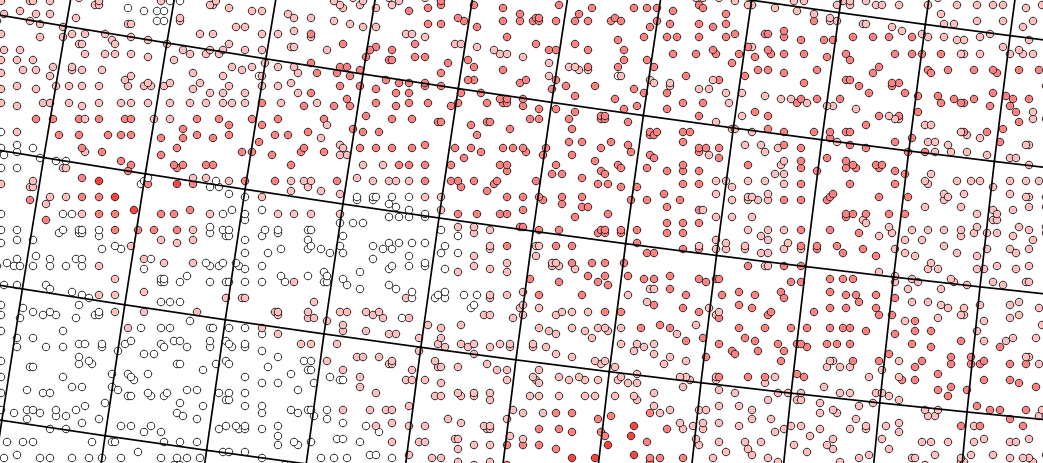
\includegraphics[width=0.9\textwidth]{figures/subgrid_scale_2d.png}
    \caption{Two dimensional example of a lot of data points per grid cell. The data points are used to compute the integral at the right hand side of \autoref{eq:disc_regularization}. \label{fig:subgrid_scale_2d}}
\end{figure}

%--------------------------------------------------------------------------------
\paragraph*{Discretization of \autoref{eq:1d_regularization}}
So the discretization of \autoref{eq:1d_regularization} with $\alpha = \frac{1}{8}$, read (i.e.\ \citet[eq.\ 7]{Borsboom1998} and \citet[eq.\ 6]{Borsboom2003}):
\begin{align}
\left( \frac{\Dx_{i-\half}}{8}
- \frac{\Psi_{i-\half}}{\Dx_{i-\half}} \right)  u_{i-1} &
+ \left( \frac{3\Dx_{i-\half}}{8}  + \frac{\Psi_{i-\half}}{{\Dx_{i-\half}}}  + \frac{3\Dx_{i+\half}}{8} +  \frac{\Psi_{i+\half}}{{\Dx_{i+\half}}} \right)  u_i +
\\
& + \left(  \frac{\Dx_{i+\half}}{8} - \frac{\Psi_{i+\half}}{{\Dx_{i+\half}}} \right)  u_{i+1}  = \int_{x_{i-1/2}}^{x_{i+\half}} u_{giv}\, dx
\label{eq:disc_regularization}
\end{align}
The boundary conditions to close the three diagonal system are $u_0  = {u_{giv}}(x_{0})$ and $u_{I+1} = {u_{giv}}(x_{I+1})$.

%--------------------------------------------------------------------------------
\subsection{Determination of artificial smoothing coefficient $\Psi$}\label{sec:determine_psi}
The artificial smoothing coefficient $\Psi$ ( $ = c_{\psi} \Dx^2 E$, \autoref{eq:regularization}) is dependent on error $E$, the smoothing coefficent $c_E$ and the second derivative of the given function $u_{giv}$ \citep[eq.\ 8]{Borsboom1998}.
The error $E$ will be computed in computational space, meaning that a disturbance is spreaded over an equal number of cells before and after the location of the disturbance:
%
\begin{align}
    &\left(\frac{\Dxi}{8}-\frac{c_E}{\Dxi}\right) E_{i-1} + \left(\frac{6\Dxi}{8} + \frac{2c_E}{\Dxi}\right) E_i + \left(\frac{\Dxi}{8} - \frac{c_E}{\Dxi}\right)E_{i+1}
    =  \int_{\xi_{i-\half}}^{\xi_{i+\half}} \abs{D_i} \, d\xi
    \label{eq:error_regularization}
\end{align}
with $\Dxi =1$ it reads:
\begin{align}
    &\left(\frac{1}{8}-c_E\right) E_{i-1} + \left(\frac{6}{8} + 2c_E\right) E_i + \left(\frac{1}{8} - c_E\right)E_{i+1}
    =   \abs{D_i}
\end{align}
\textbf{Choose $\mathbf{c_E}$ equal to $\mathbf{c_{\psi}}$} and take into account that $D_i$ is constant over a control volume
\begin{align}
    D_i & = \Dxi^2 \pdiff[2]{u_{giv}}{\xi} \quad \text{ \citep[eq.\ 2]{Borsboom1998}}
    \\ & \approx {u_{giv}}_{i-1} - 2 {u_{giv}}_{i-1} + {u_{giv}}_{i+1}
\end{align}
%
Now system the system of \autoref{eq:error_regularization} can be solved and where $\vec{\Psi}$ is set to:
\begin{align}
    \vec{\Psi} = c_{\Psi}\Dx^2 \vec{E}
\end{align}
For an estimation of $c_{\Psi}$ see \autoref{sec:determine_factor_c_psi}, in this document we use $c_{\Psi} = 4$.

The boundary conditions to close the three diagonal system are:
\begin{align}
    2 E_0 - E_1 & = \abs{D_{1}} \quad \text{and}
    \\
    - E_{I} + 2 E_{I+1} & = \abs{D_{I}}.
\end{align}

%--------------------------------------------------------------------------------
\subsection{Step function (Heaviside function)}
For a full description of this example see \citet[eq.\ 5]{Borsboom2003}.
The function is initially defined as:
\begin{align}
    u_{given}(x) =
    \begin{cases}
        0, & \text{if} \quad 0\ [m] \leq x \leq 1000\ [m],
        \\
        1, & \text{if} \quad 1000\ [m] < x \leq 2000 \ [m],
    \end{cases}
\end{align}
For illustration, the step is chosen to be exactly on a grid point (in the middle of a control volume at $1000\ [m]$) and at the finite volume boundary, i.e.\ a half $\Dx$ shifted to the right.
\begin{figure}[H]
    \centering
    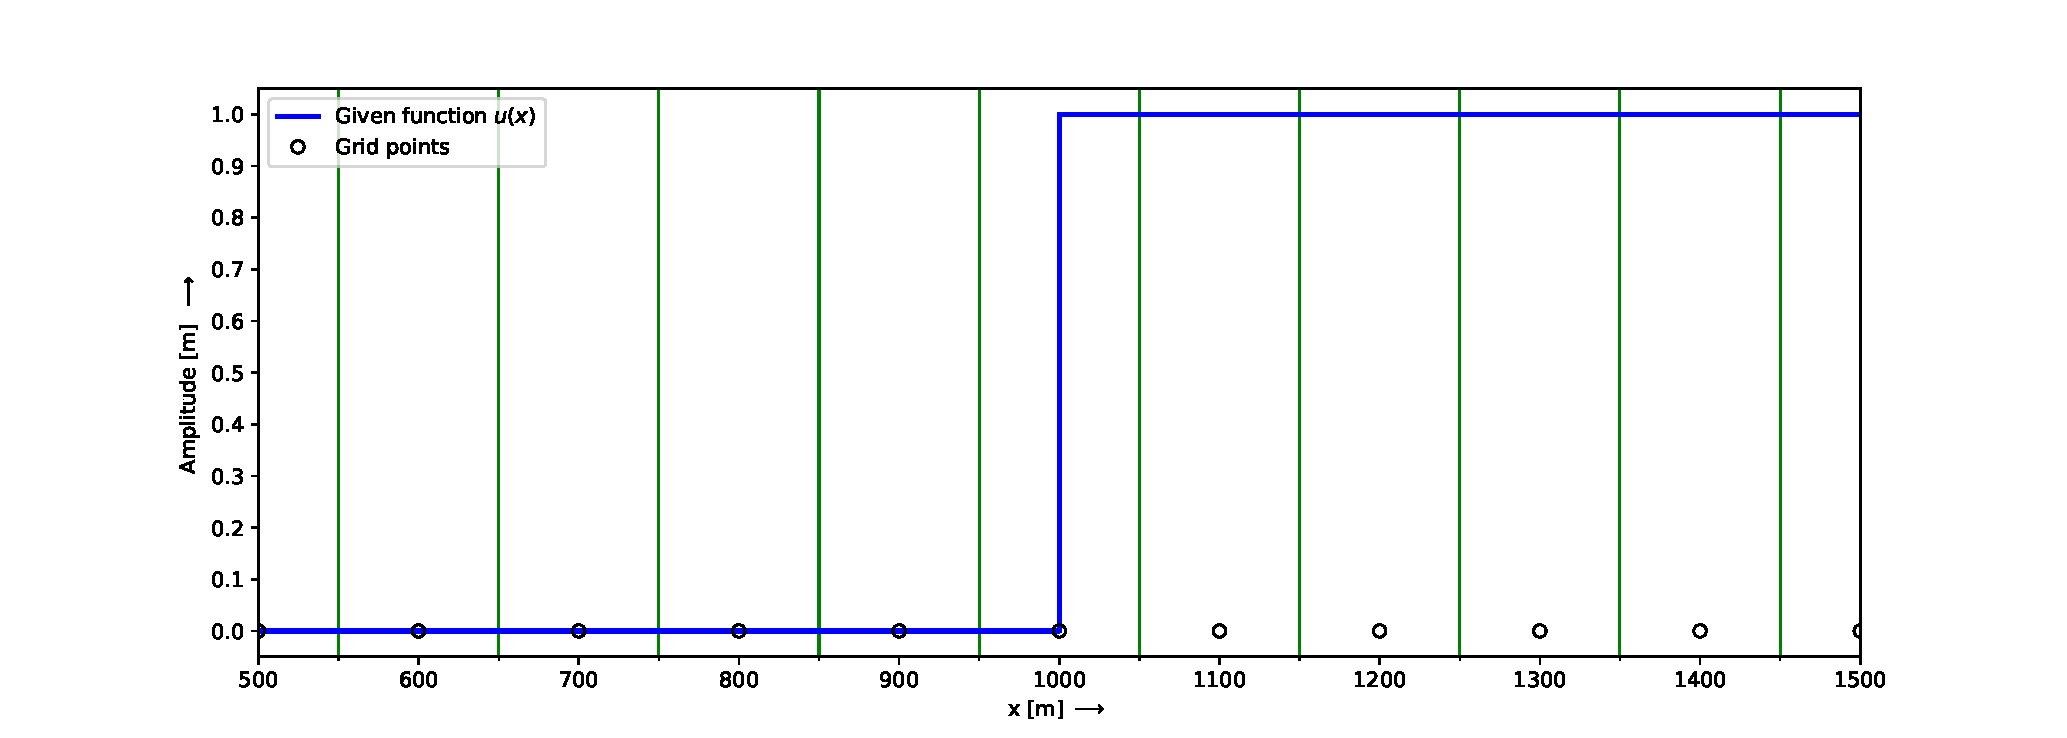
\includegraphics[width=1.0\textwidth]{figures/1d_step_function_dx100.pdf}
    \caption{Step function to be estimated. The thin green vertical lines indicate the  borders of the finite volumes.\label{fig:ex_step_function}}
\end{figure}
A straight forward piecewise approximation is shown in \autoref{fig:straight_forward_discretization}.
Both figures does show the same discretization function (cyan colored) but the step is at a different location.
%
\begin{figure}[H]
    \centering
    \begin{subfigure}[t]{0.49\textwidth}
        \centering
        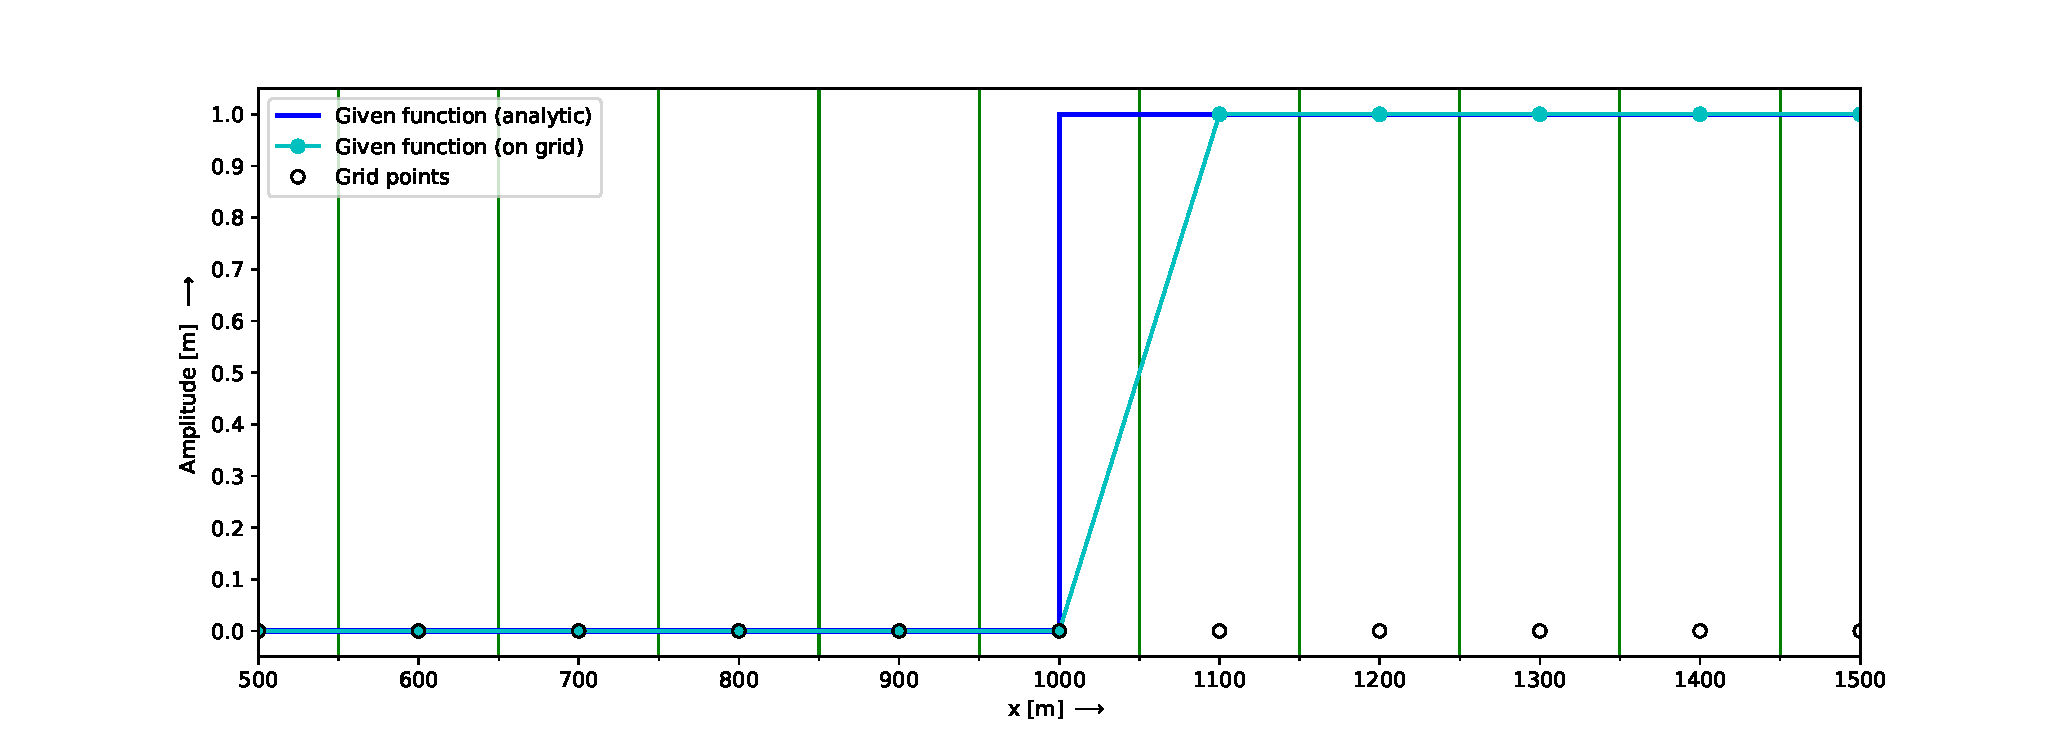
\includegraphics[width=1.0\textwidth]{figures/regul_1_1d_scalar_dx100.pdf}
        \caption{Step at grid node, $x = 1000\ [m]$}
    \end{subfigure}
    \hfill
    \begin{subfigure}[t]{0.49\textwidth}
        \centering
        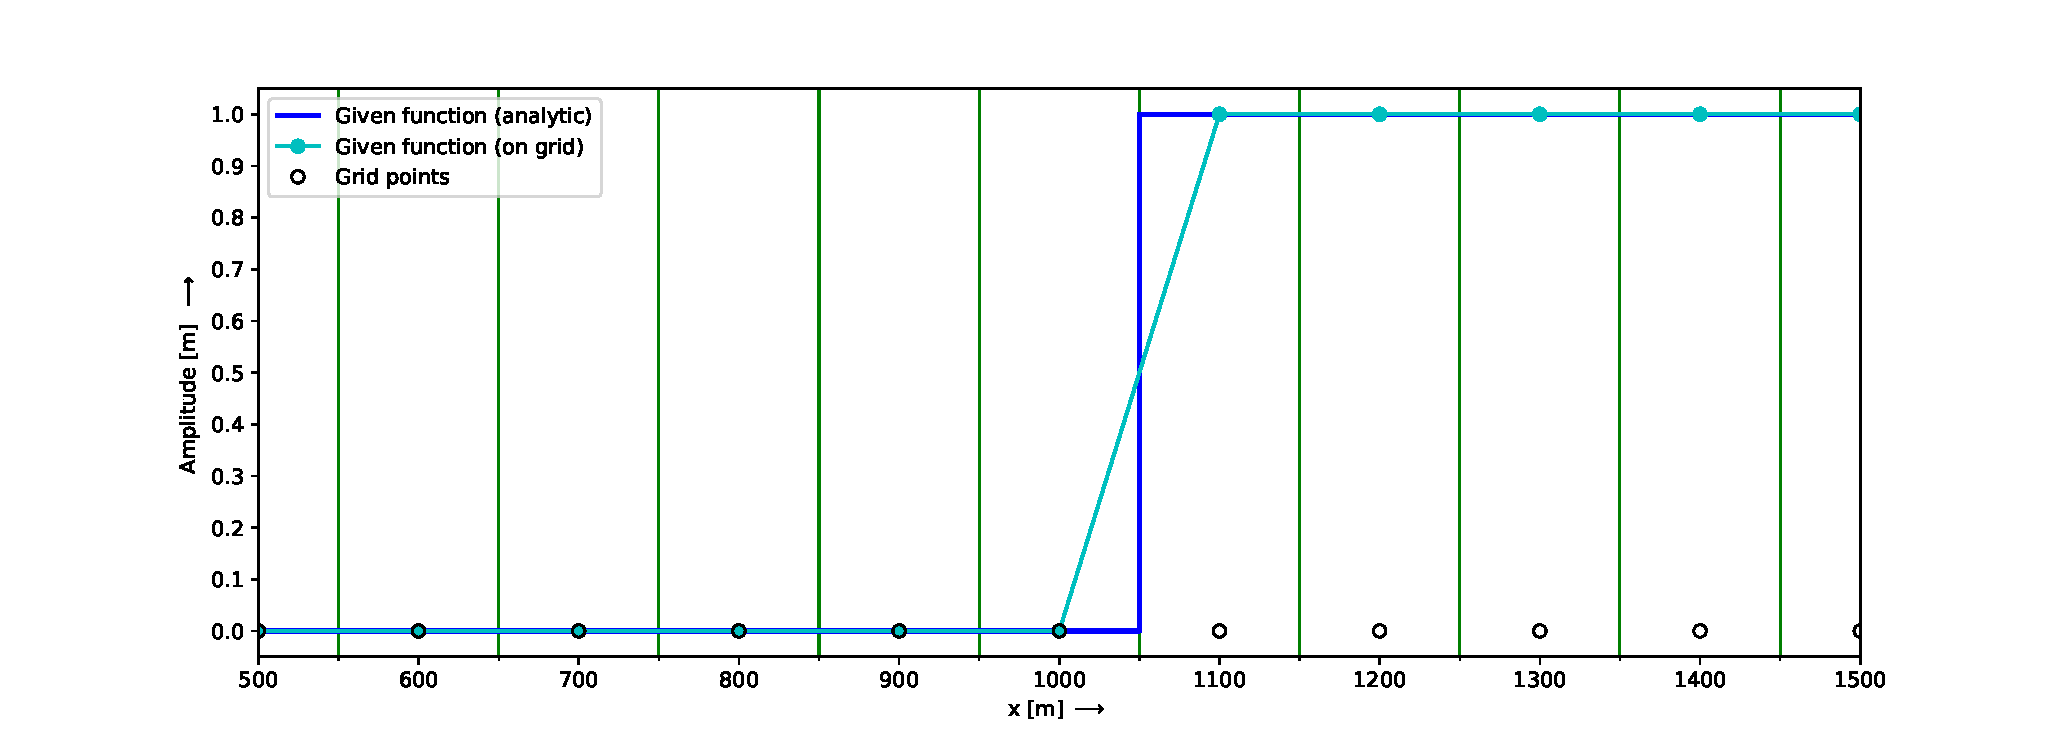
\includegraphics[width=1.0\textwidth]{figures/regul_2_1d_scalar_dx100.pdf}
        \caption{Step at boundary of a finite volume, $x = 1050\ [m]$}
    \end{subfigure}
    \caption{As seen from this figures the function defined on the grid nodes does not see the exact location of the step. Both functions through the grid nodes have the same profile, but the step is at another location. \label{fig:straight_forward_discretization}}
\end{figure}
%
A piecewise approximation with a regularization coefficient of zero ($c_\Psi = 0$) is shown in \autoref{fig:ex_step_function_no_regularization}.
%
\begin{figure}[H]
    \centering
    \begin{subfigure}[t]{0.49\textwidth}
        \centering
        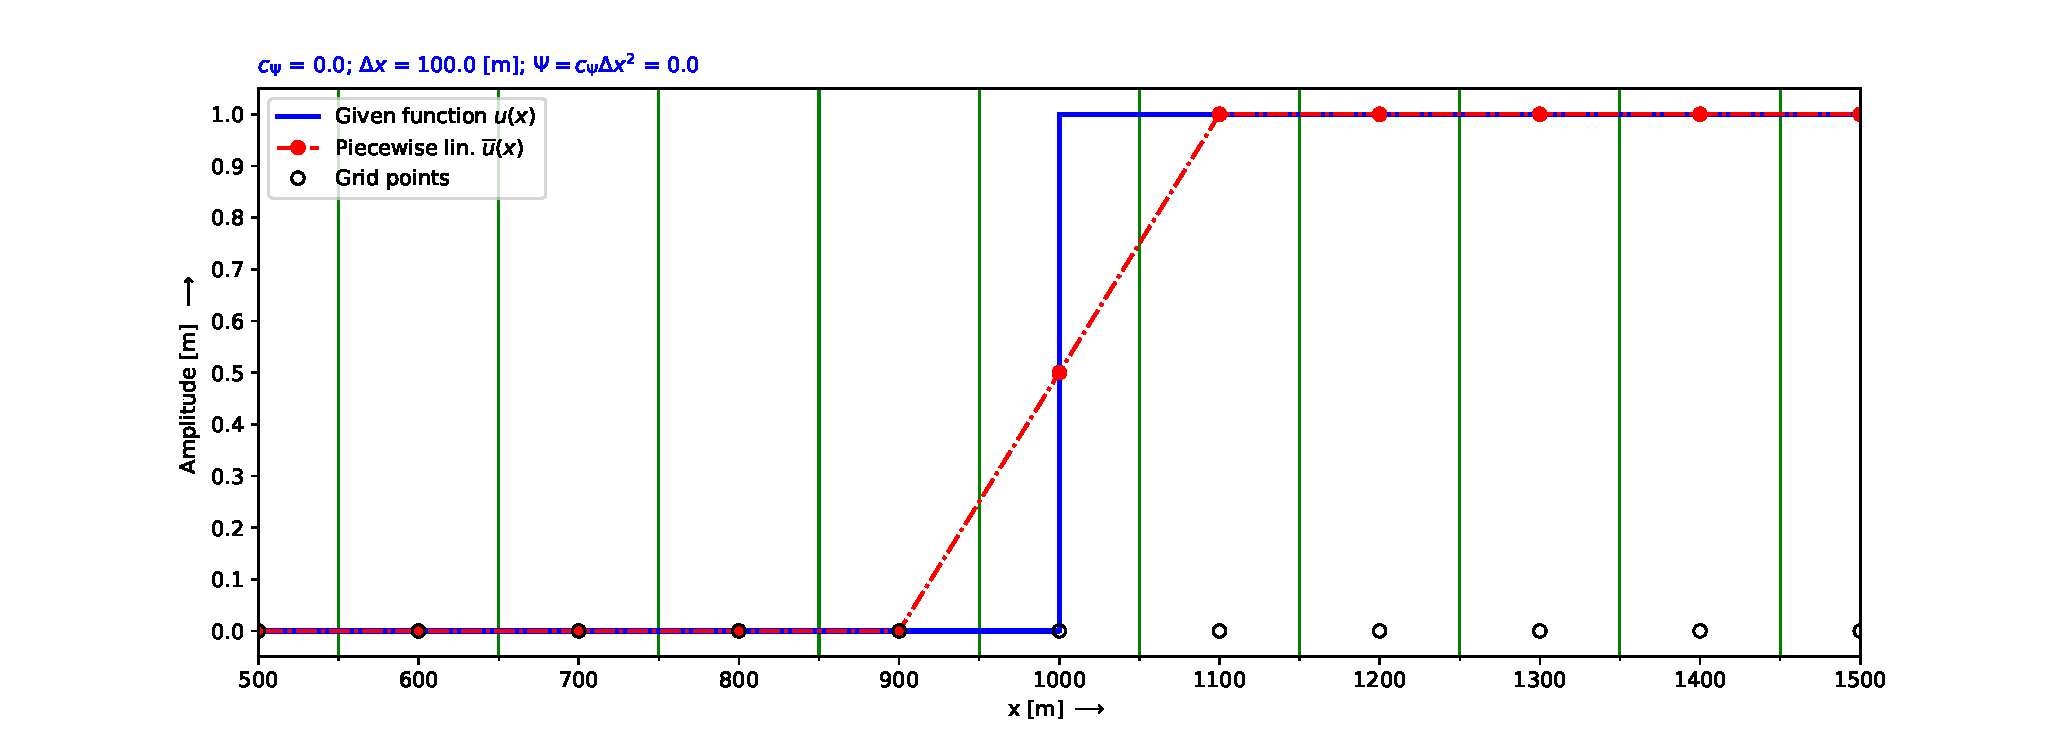
\includegraphics[width=1.0\textwidth]{figures/regul_1_1d_step_function_dx100.0_cpsi1e-06.pdf}
        \caption{Step at grid node, $x = 500\ [m]$}\label{fig:ex_step_function_no_regularization_a}
    \end{subfigure}
    \hfill
    \begin{subfigure}[t]{0.49\textwidth}
        \centering
        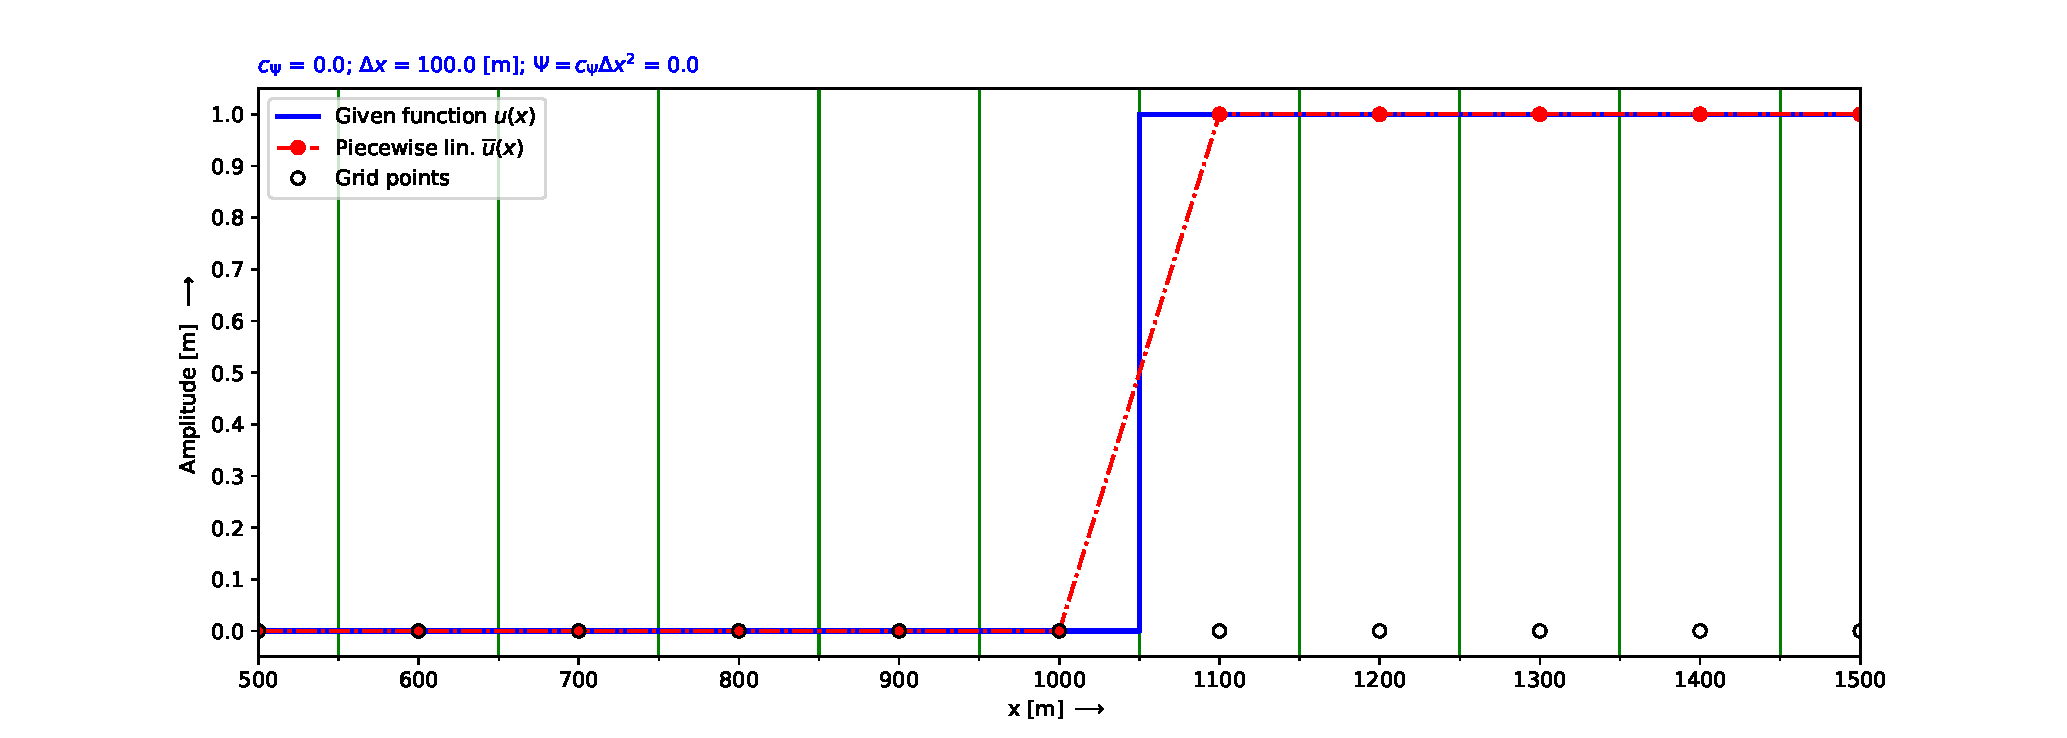
\includegraphics[width=1.0\textwidth]{figures/regul_2_1d_step_function_dx100.0_cpsi1e-06.pdf}
        \caption{Step at boundary finite volume, $x = 550\ [m]$}\label{fig:ex_step_function_no_regularization_b}
    \end{subfigure}
    \caption{Step function approximated by a piecewise linear function (red line with dots at the nodes), $c_{\Psi} = 0$, $\Dx = 100\ [m]$ and $\Psi = 0$. The thin green vertical lines indicate the  borders of the finite volumes. \label{fig:ex_step_function_no_regularization}}
\end{figure}
As seen from  \autoref{fig:ex_step_function_no_regularization} the step is more taken into account as is presented in \autoref{fig:straight_forward_discretization}.
Which looks quite well, but what are the values of the second derivative of the solution.
For $\Dx=\SI{100}{[\metre]}$ the absolute value of the second derivative is $0.5/(100)^2$ (\autoref{fig:ex_step_function_no_regularization_a}) and $1.0/(100)^2$ (\autoref{fig:ex_step_function_no_regularization_b}).


There are two options to estimate this step function by a piecewise linear smooth function with the same numerical accuracy:
\begin{enumerate}
    \item Regularization with using a large grid size, the numerical solution is less close to the step function (see \autoref{fig:ex_step_function_larger_dx})
    \item Regularization with using a small grid size, the numerical solution is closer to the step function (see \autoref{fig:ex_step_function_smaller_dx}),
\end{enumerate}
Both options has the same value for $c_{\Psi} = 4$. Meaning that the step is represented by the same number of grid cells.
How to estimate $c_\Psi$ can be read in \autoref{sec:error_estimation}.
It is up to the user which regularization is can be used for the numerical simulation.
A better representation of the step function need a smaller grid size.
\begin{figure}[H]
    \centering
    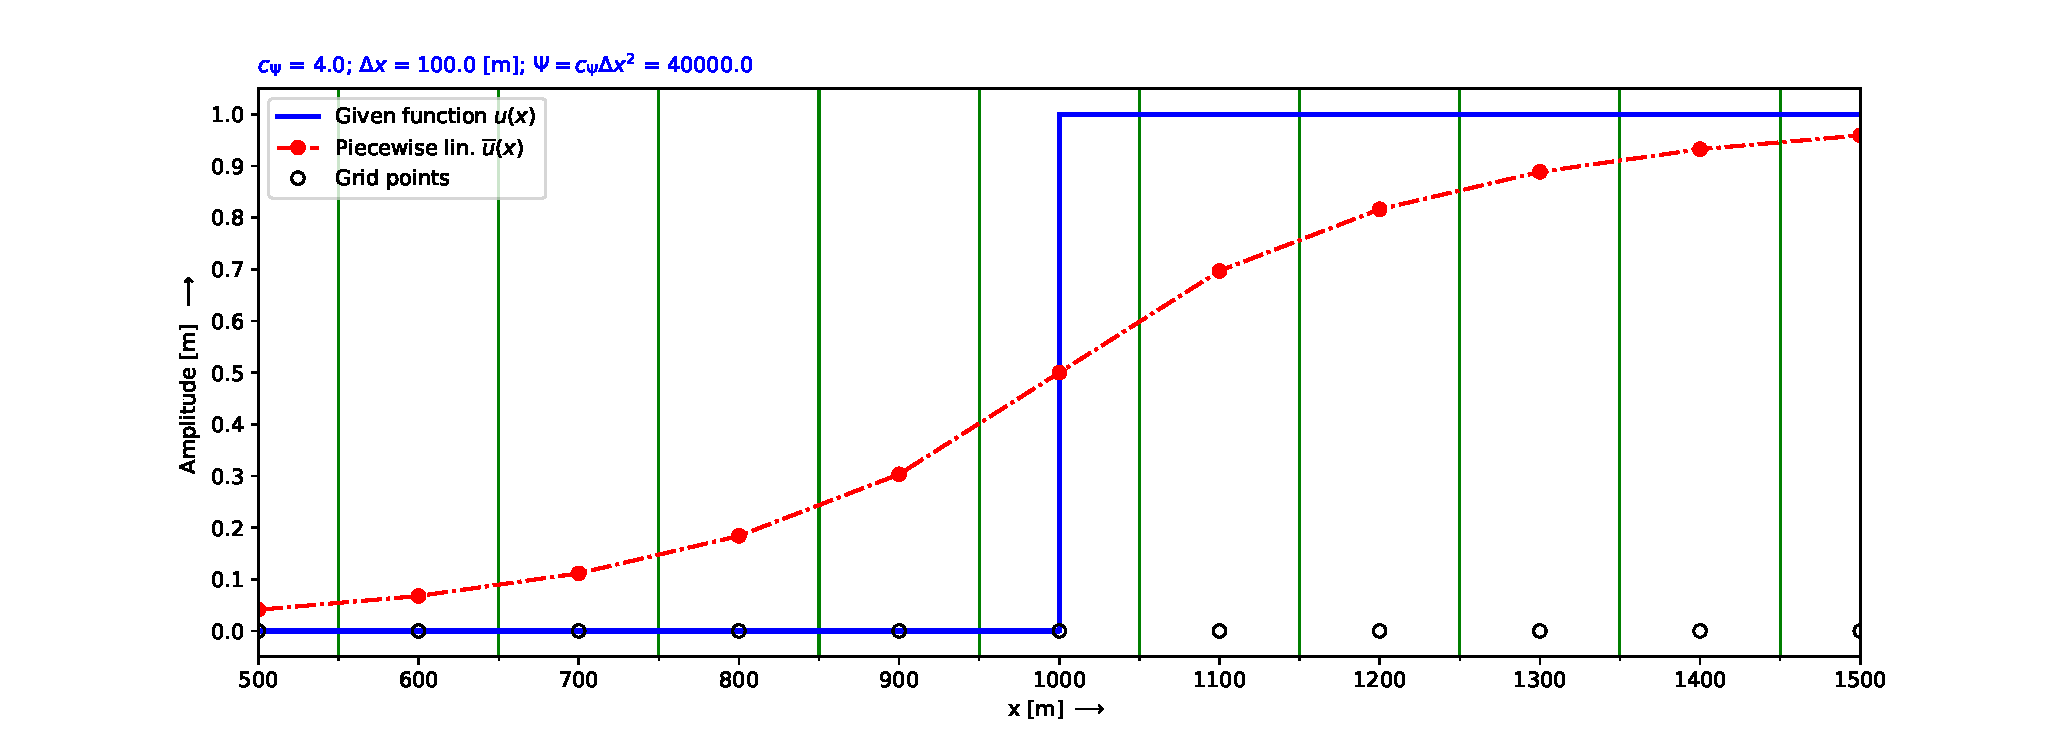
\includegraphics[width=1.0\textwidth]{figures/regul_1d_step_function_dx100.0_cpsi4.0.pdf}
    \caption{Step function approximated by a piecewise linear function (red line with dots at the nodes), $c_{\Psi} = 4$, $\Dx = 100\ [m]$ and $\Psi = 40000$. The thin green vertical lines indicate the  borders of the finite volumes. \label{fig:ex_step_function_larger_dx}}
\end{figure}
\begin{figure}[H]
    \centering
    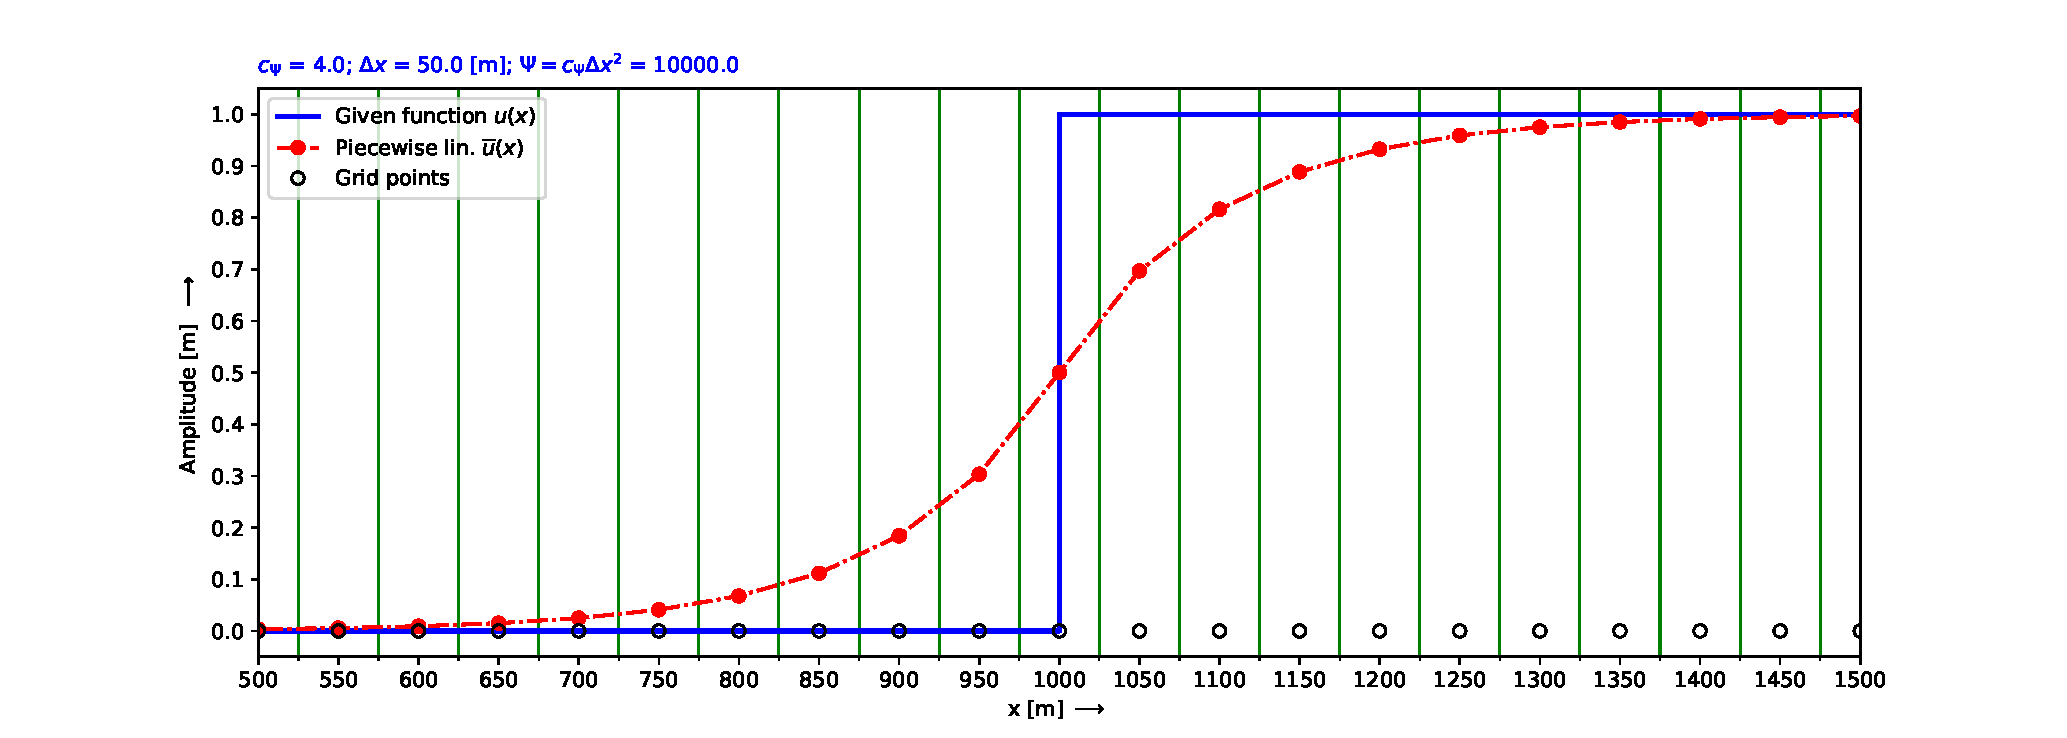
\includegraphics[width=1.0\textwidth]{figures/regul_1d_step_function_dx50.0_cpsi4.0.pdf}
    \caption{Step function approximated by a piecewise linear function (red line with dots at the nodes), $c_{\Psi} = 4$, $\Dx = 50\ [m]$ and $\Psi =10000$. The thin green vertical lines indicate the  borders of the finite volumes. \label{fig:ex_step_function_smaller_dx}}
\end{figure}
\vspace*{0.5\baselineskip}
%
%--------------------------------------------------------------------------------
\subsection{Small and a large gradient in the data set}
To show the influence of  regularization a more general data set is chosen, \citet{Borsboom1998} (given function, here adjusted).
A given function  with a small (smooth) and large  (steep) gradients in the data set is chosen.
The function is defined by:
\begin{align}
u_{given}(x) =
\begin{cases}
    10 \left(\half - \half \tanh{(20x/1000-6)}\right), & \text{if} \quad 0\ [m] \leq x \leq 650\ [m],
    \\
    10, & \text{if} \quad 650\ [m] < x \geq 1000 \ [m],
\end{cases}
\end{align}
and shown in \autoref{fig:tanh_step}:
\begin{figure}[H]
    \centering
    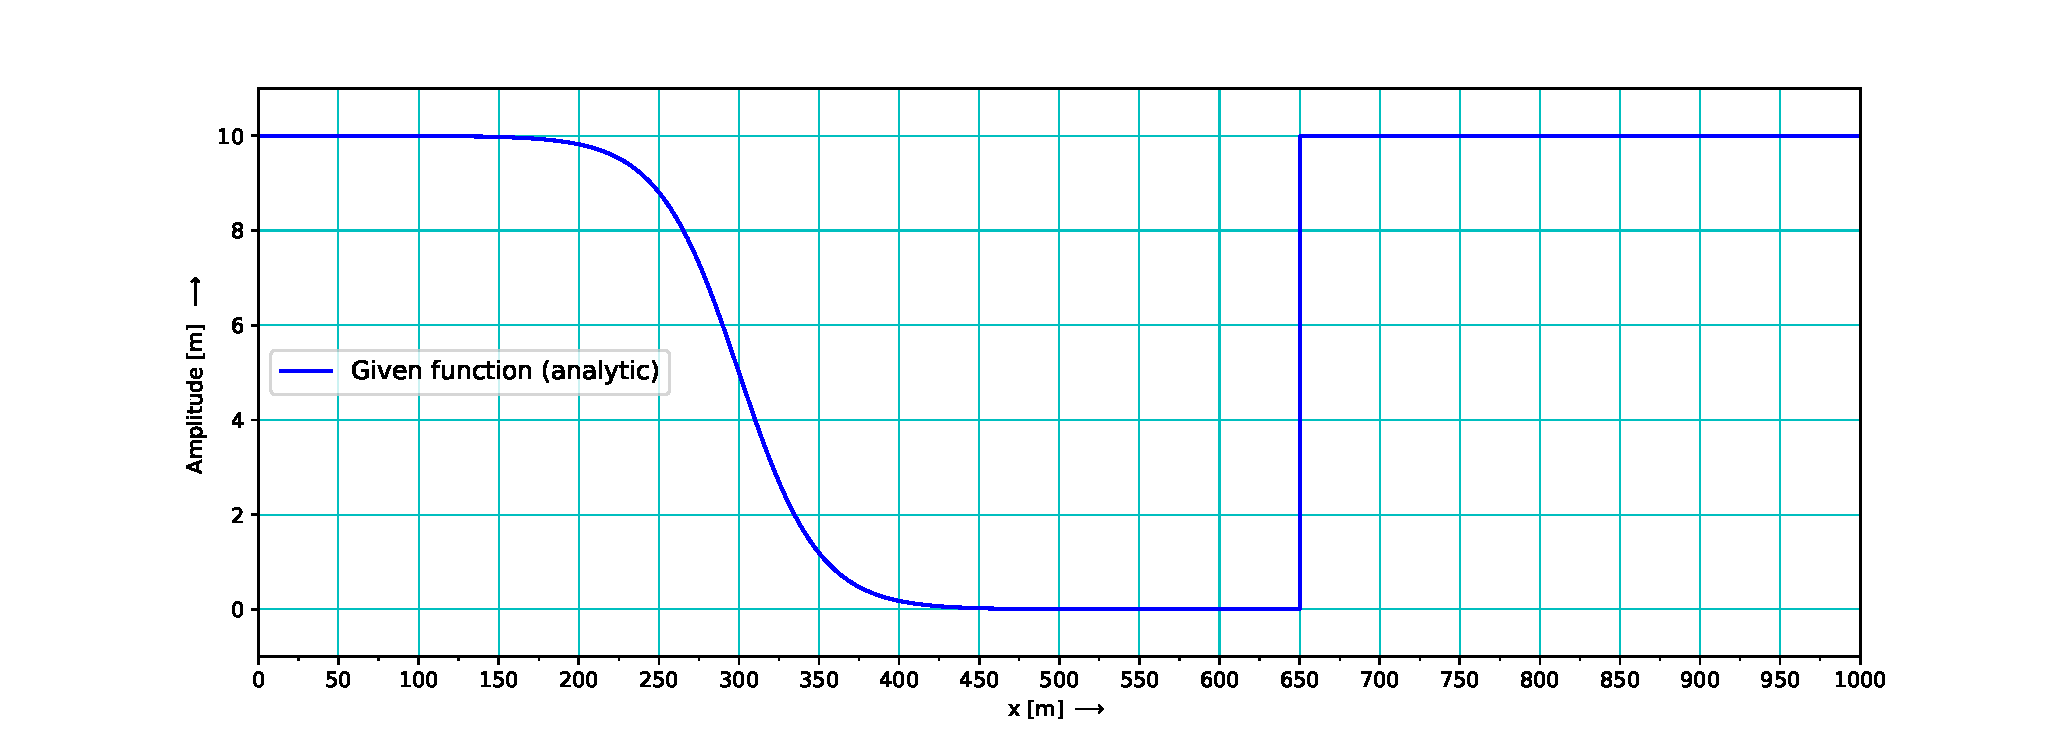
\includegraphics[width=1.0\textwidth]{figures/regul_tanh_step.pdf}
    \caption{Large and small gradients in given function. \label{fig:tanh_step}}
\end{figure}

First guess of regularization:
\begin{figure}[H]
    \centering
    \begin{subfigure}[t]{0.49\textwidth}
    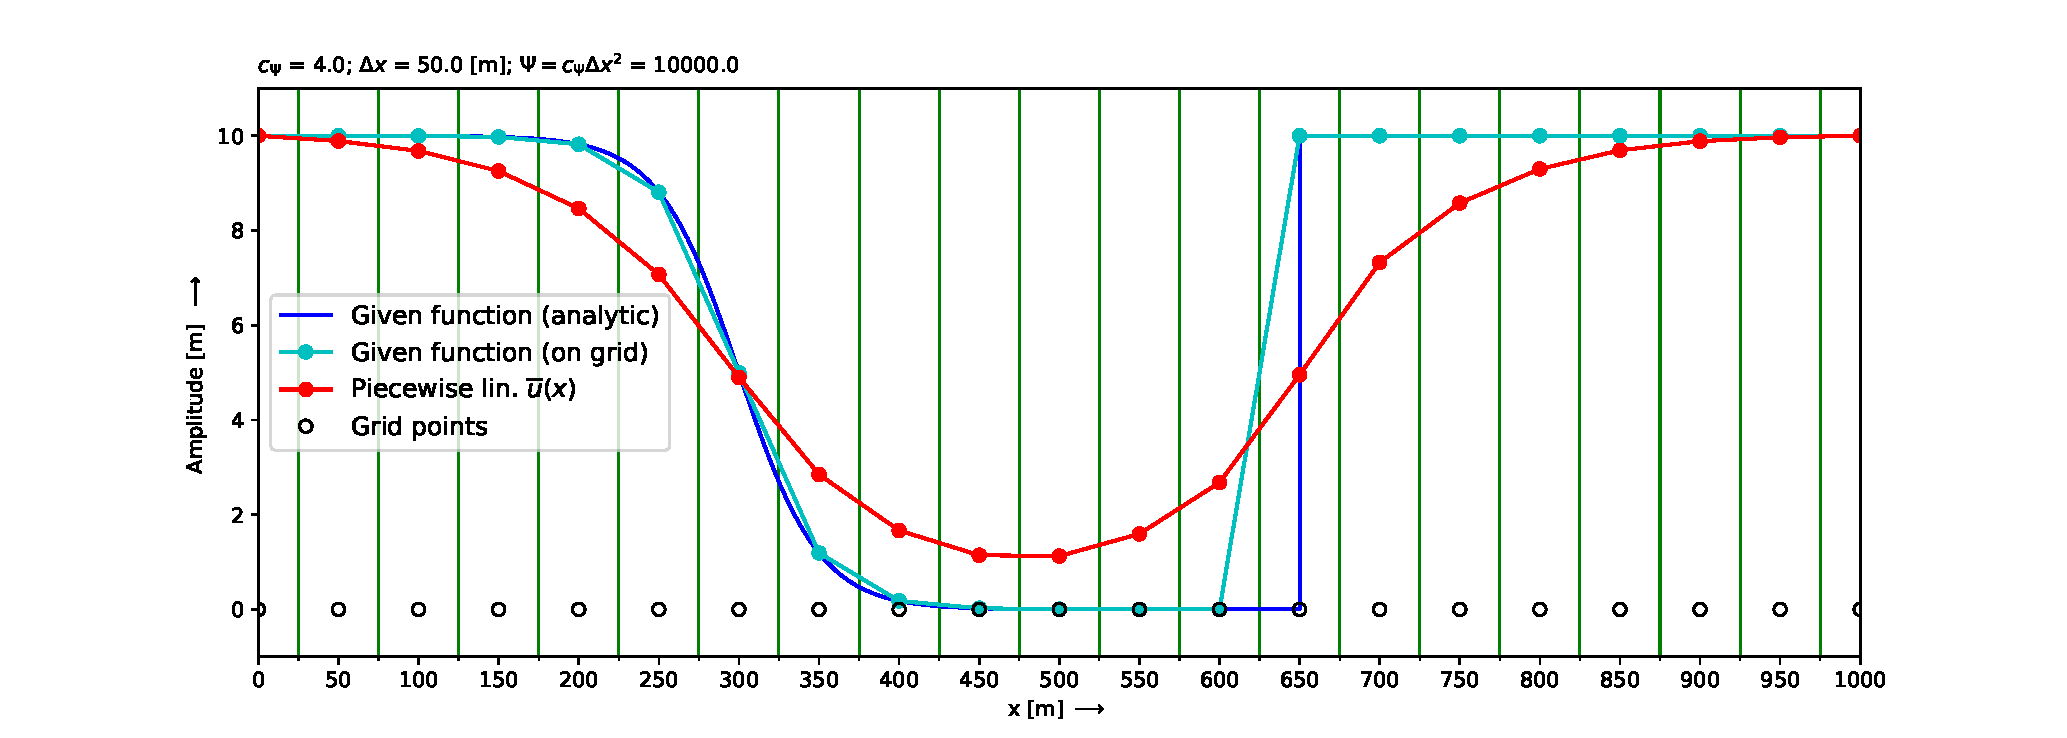
\includegraphics[width=1.0\textwidth]{figures/regul_1_1d_scalar_dx50.0_cpsi4.0.pdf}
\caption{Grid size $\Dx = 50\ [m]$}
    \end{subfigure}
    \hfill
    \begin{subfigure}[t]{0.49\textwidth}
        \centering
        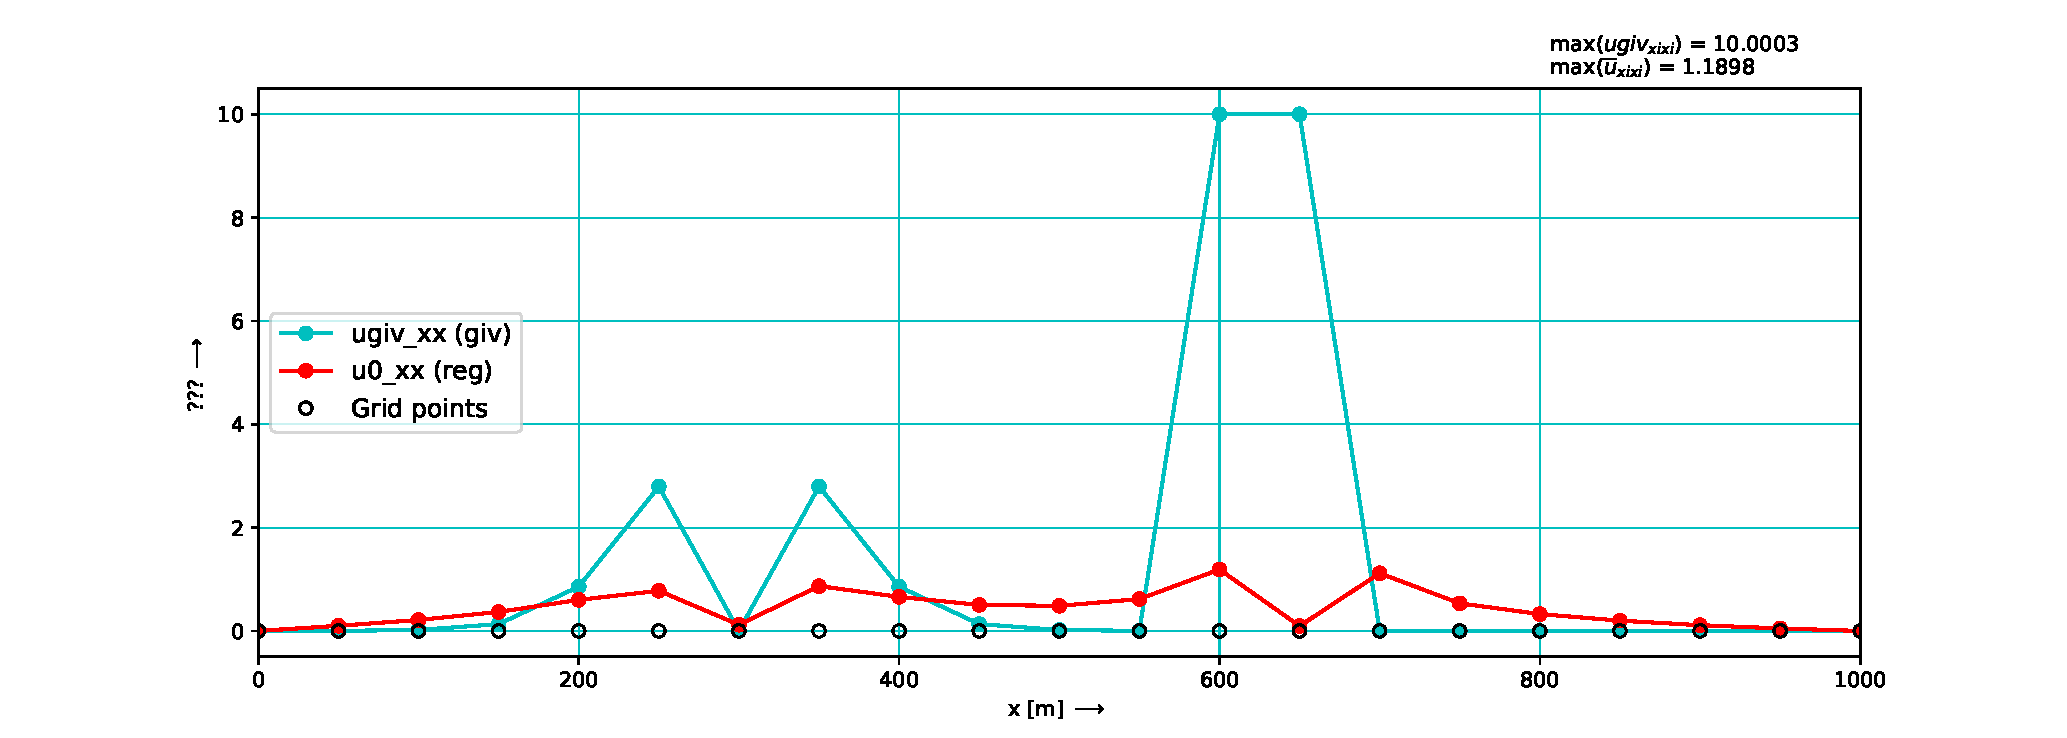
\includegraphics[width=1.0\textwidth]{figures/regul_2_1d_scalar_dx50.0_cpsi4.0.pdf}
        \caption{Second derivatives, normalized grid size $\Dxi = 1$.}
    \end{subfigure}
    \caption{Initial guess ($c_\Psi = 4, \Dx = 50\ [m]$)}
\end{figure}

There are two options to adjust the data:
\begin{enumerate}
    \item increase the regularization coefficient or
    \item choose a smaller grid size.
\end{enumerate}
%--------------------------------------------------------------------------------
\paragraph*{Regularization coefficient increased}
Increasing the regularization coefficient $c_\Psi$:
\begin{figure}[H]
    \centering
    \begin{subfigure}[t]{0.49\textwidth}
        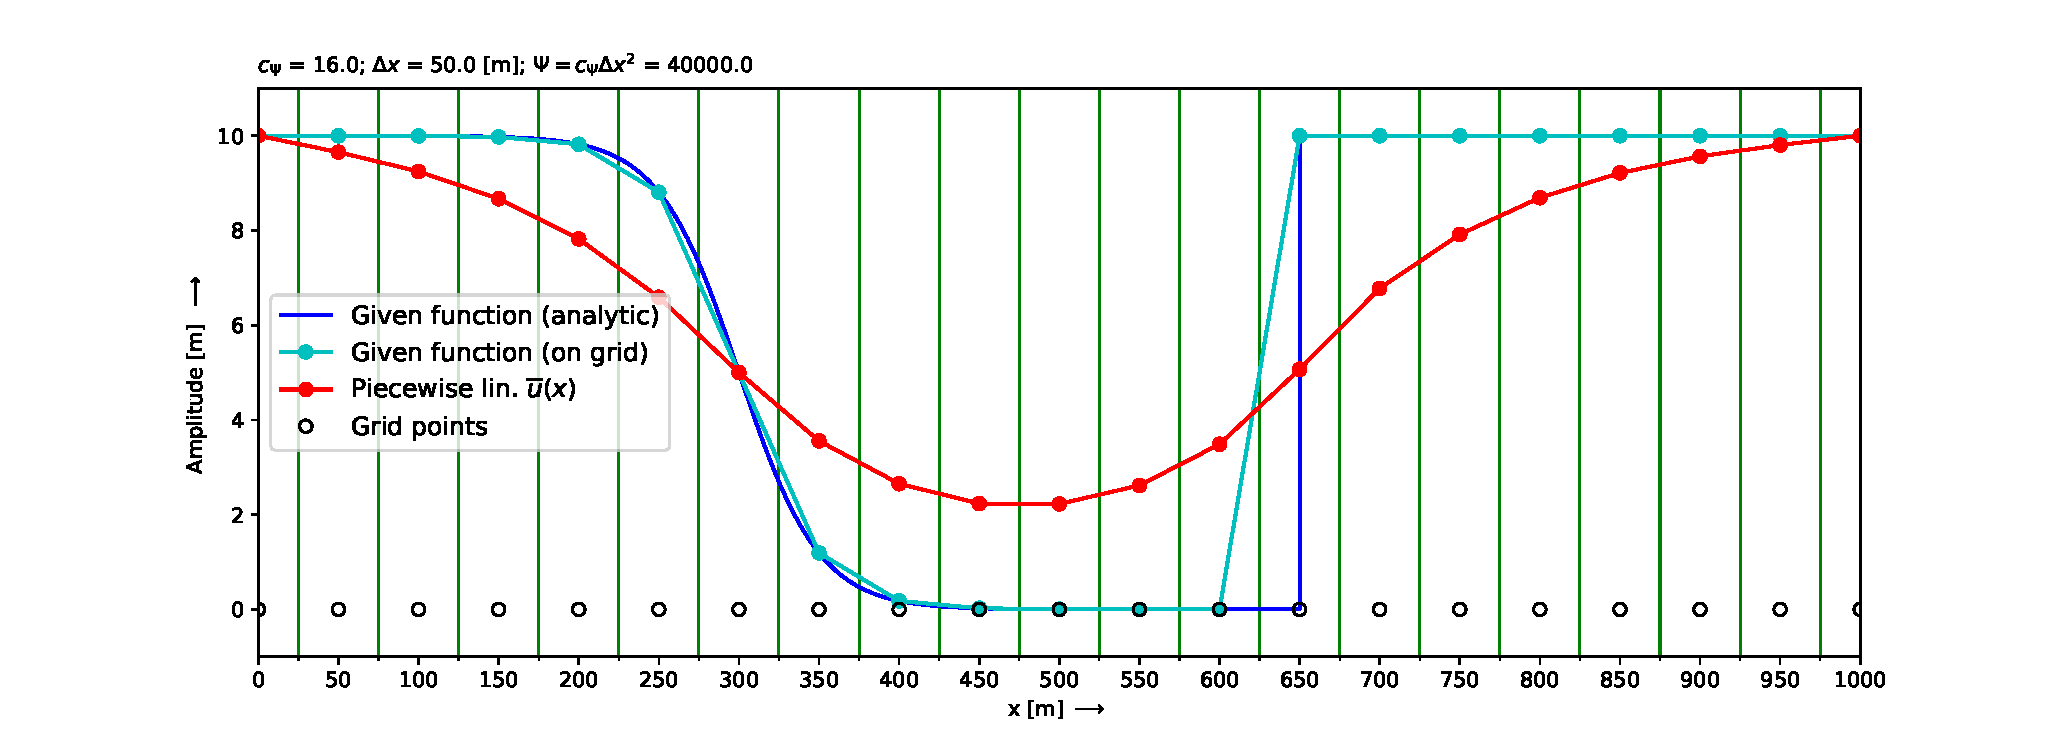
\includegraphics[width=1.0\textwidth]{figures/regul_1_1d_scalar_dx50.0_cpsi16.0.pdf}
        \caption{Grid size $\Dx = 50\ [m]$}
    \end{subfigure}
    \hfill
    \begin{subfigure}[t]{0.49\textwidth}
        \centering
        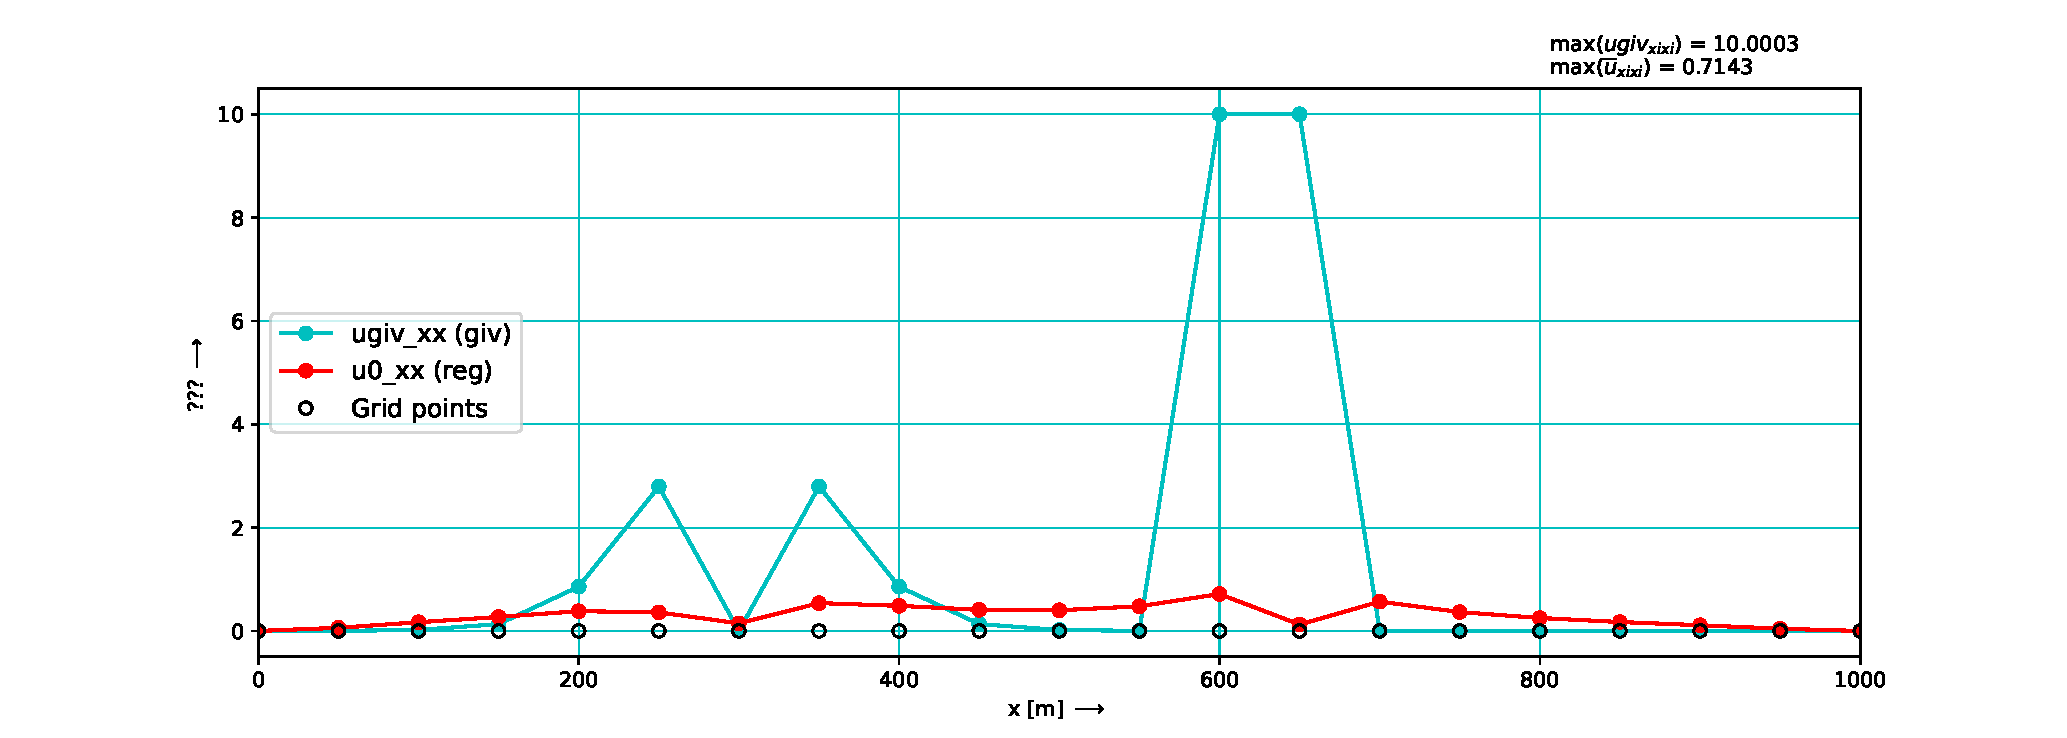
\includegraphics[width=1.0\textwidth]{figures/regul_2_1d_scalar_dx50.0_cpsi16.0.pdf}
        \caption{Second derivatives, normalized grid size $\Dxi = 1$.}
    \end{subfigure}
    \caption{Regularization coefficient increased to 16 ($c_\Psi = 16, \Dx = 50\ [m]$)}
\end{figure}
%--------------------------------------------------------------------------------
\paragraph*{Grid size decreased}
Decrease the grid size $\Dx$:
\begin{figure}[H]
    \centering
    \begin{subfigure}[t]{0.49\textwidth}
        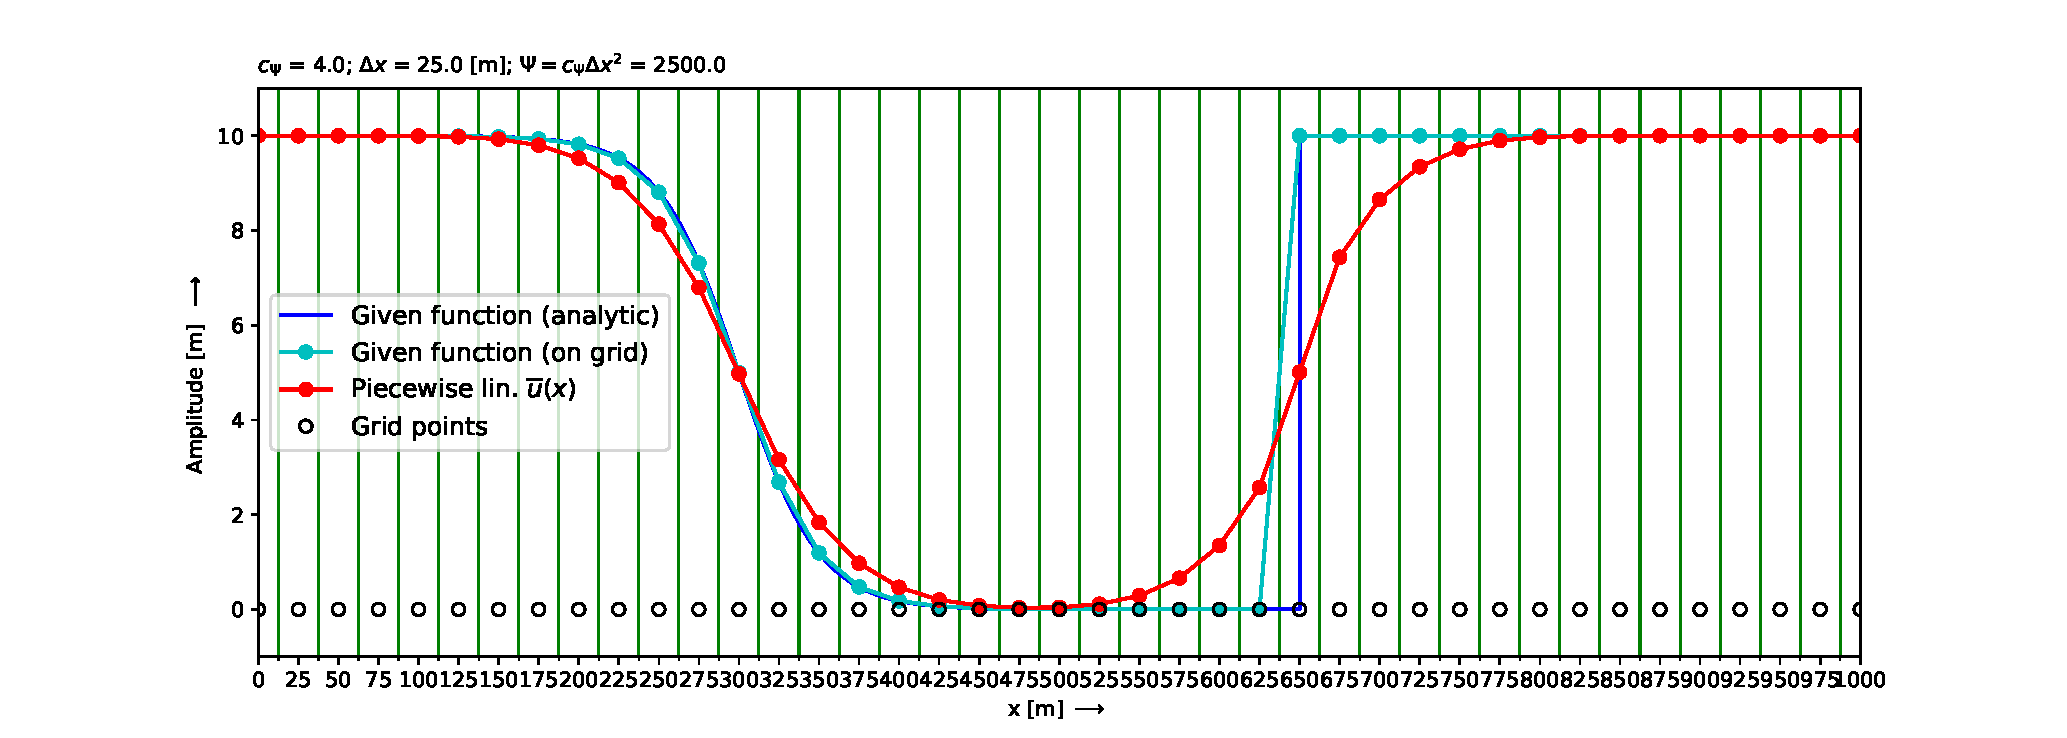
\includegraphics[width=1.0\textwidth]{figures/regul_1_1d_scalar_dx25.0_cpsi4.0.pdf}
        \caption{Step at grid node, $c_\Psi = 4, \Dx = 25\ [m]$}
    \end{subfigure}
    \hfill
    \begin{subfigure}[t]{0.49\textwidth}
        \centering
        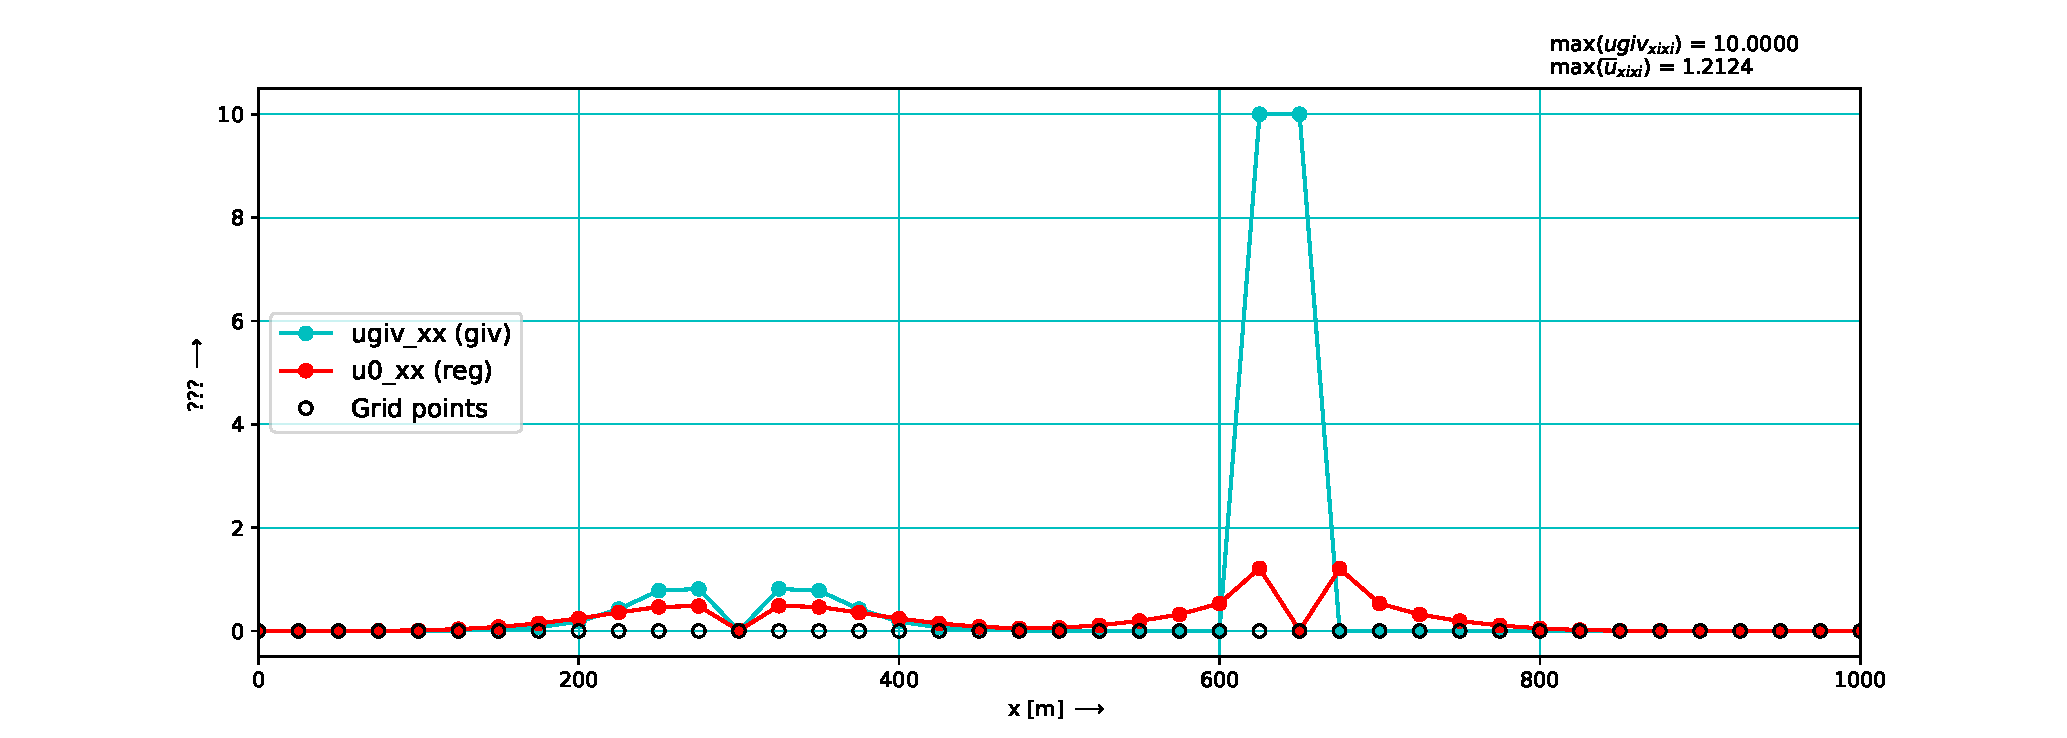
\includegraphics[width=1.0\textwidth]{figures/regul_2_1d_scalar_dx25.0_cpsi4.0.pdf}
        \caption{Second derivatives.}
    \end{subfigure}
    \caption{Grid size decreased to $25\ [m]$ ($c_\Psi = 4, \Dx = 25\ [m]$)}
\end{figure}
%------------------------------------------------------------------------------
\section{Compatible initialization in one dimension}\label{sec:compatible_initialization}
To assure that the given initial condition(s) are compatible with the numerical scheme, the given function need to fulfill the follow equation:
\begin{align}
    \int_{x_{i-\half}}^{x_{i+\half}} \overline u_{initial}\, dx = \int_{x_{i-\half}}^{x_{i+\half}} u_{given}\, dx \label{eq:compatible_initialization}
\end{align}
where $\overline{u}$ is the piecewise linear function and $u_{given}$ the given initial condition.
In case the function $u_{given}$ is an integrable analytic function the integral can be exact computed.
In discrete form the equation for each control volume reads:
\begin{align}
    \frac{\Dx_{i-\half}}{2}\,\frac{u_{i-1} + 3 u_i}{4} +
    \frac{\Dx_{i+\half}}{2}\,\frac{3 u_i + u_{i+1}}{4} = \int_{x_{i-\half}}^{x_{i+\half}} u_{given}\, dx
\end{align}
Extra equations are needed for the boundary conditions, the following boundary treatment is used at $x=0$ (see  \autoref{sec:boundary_conditions}):
\begin{align}
    \frac{1}{12} u_0 + \frac{10}{12}u_1 + \frac{1}{12} u_2 = u_{given}(0)
\end{align}
and similar at the other boundary ($x=12$).
An illustration off the result of \autoref{eq:compatible_initialization} is given in \autoref{fig:compatible_initial_condition}.
\begin{figure}[H]
    \centering
    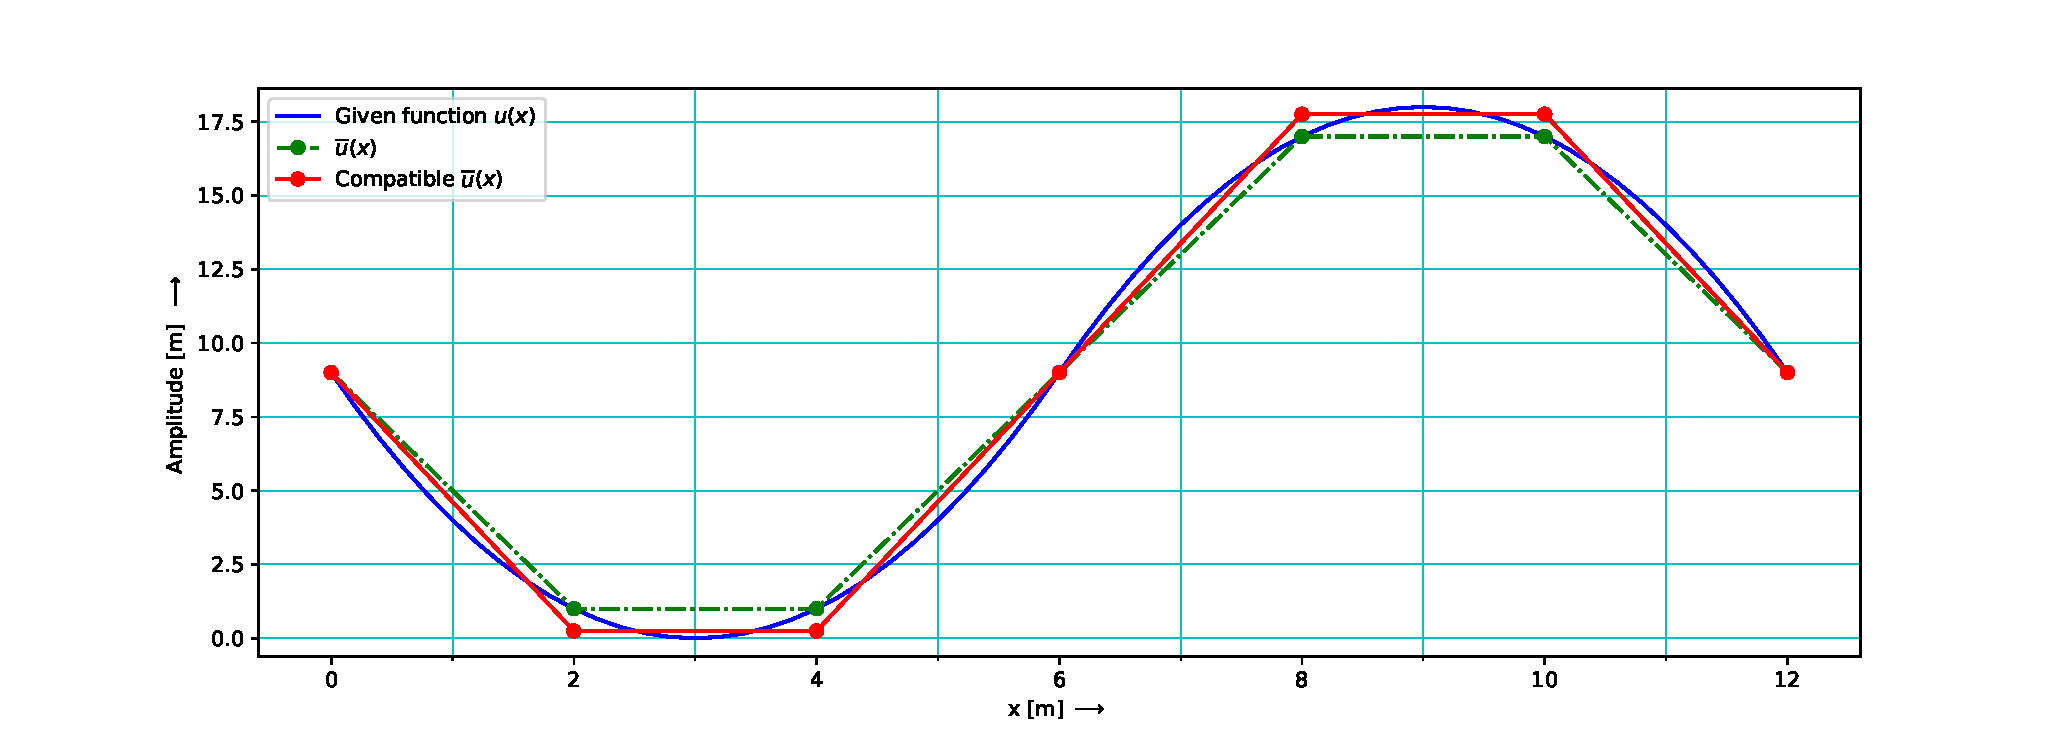
\includegraphics[width=0.9\textwidth]{figures/compatible_initialization_lx=12.0_dx=2.0.pdf}
    \caption[Illustration of compatible quadratic function]{
    Illustration of compatible quadratic function.
    The integral over the control volume of the the given function (blue) is equal represented by the red-function and better then by the green-function, therefor the red function is called compatible with the given function.
    The green-function is defined with nodes on the given function. Control volumes shown by the green vertical lines.
    And the gray areas are virtual and are not belonging to the water body (see \autoref{fig:water_body_fve_bc_at_node}). }\label{fig:compatible_initial_condition}
    % python script: compatible_initial_function.py
\end{figure}
Some numerical items used to generate \autoref{fig:compatible_initial_condition} are $x \in [0, 12]$, $\Dx=2$ and the given function reads:
\begin{align}
    &u_{given}(x) =
    \begin{cases}
        (x-3)^2 & \qquad x < 6
        \\
        -(x-3)^2 + 18 & \qquad x \geq 6
    \end{cases}
\end{align}
%------------------------------------------------------------------------------
\section{Compatible initialization in two dimensions}\label{sec:compatible_initialization}
To assure that the given initial condition(s) are compatible with the numerical scheme, the given function need to fulfill the follow equation for each control volume:
\begin{align}
    \int_{y_{i-\half}}^{x_{i+\half}} \int_{y_{i-\half}}^{x_{i+\half}} \overline u_{initial}\, dxdy = \int_{y_{i-\half}}^{y_{i+\half}} \int_{x_{i-\half}}^{x_{i+\half}} u_{given}\, dxdy \label{eq:compatible_initialization}
\end{align}
where $\overline{u}$ is the piecewise linear function and $u_{given}$ the given initial condition.
See for an example \autoref{fig:subgrid_scale_2d}, when the function $u_{given}$ is constructed by an interpolation method (triangulation, \ldots) between the dots.
In case the function $u_{given}$ is an integrable analytic function the integral can be exact computed.

On a structured grid one control volume ($cv$) around a node consist of four sub-control volumes ($scv_i$, $i\in\{1,2,3,4\}$).
\begin{align}
    &\int_{scv_1} \overline u_{initial}\, d\omega +
    \int_{scv_2} \overline u_{initial}\, d\omega +
    \int_{scv_3} \overline u_{initial}\, d\omega +
    \int_{scv_4} \overline u_{initial}\, d\omega
    =
    \nonumber \\
    & =\int_{scv_1} u_{given}\, d\omega +
    \int_{scv_2} u_{given}\, d\omega +
    \int_{scv_3} u_{given}\, d\omega +
    \int_{scv_4} u_{given}\, d\omega
\end{align}

Considering one sub-control volume, $scv_3$, and assuming a
cartesian grid then the discrete form reads :
\begin{align}
A_{scv_3} \overline{u}_{qp} = \int_{scv_3} u_{given}\, d\omega
\end{align}
with $A_{scv_3} \approx \Dx_{qp}\Dy_{qp}$ the area of sub-control volume $scv_3$, with
\begin{align}
    \Dx_{qp} & = \frac{1}{2}\left[\frac{1}{4}\left( 3 (x_{i+1,j} - x_{i,j}) + 1 (x_{i+1,j+1} - x_{i,j+1}) \right)\right],
    \\
    \Dy_{qp} & = \frac{1}{2}\left[\frac{1}{4}\left( 3 (y_{i+1,j} - y_{i,j}) + 1 (y_{i+1,j+1} - yx_{i,j+1}) \right)\right],
    \\
    \overline{u}_{qp} & = \frac{1}{16} \left( 9 u_{i,j} + 3 u_{i+1,j} + 3 u_{i, j+1} + u_{i+1, j+1} \right).
\end{align}

